\apendice{Especificación de Requisitos}

Un stakeholder es cualquier persona u organización interesada, afectada o implicada en el funcionamiento del software que se desarrolla \\ \cite{pradel2013ingenieria}. Van a desempeñar un papel clave y activo en la especificación y validación de los requerimientos del software \\ \cite{oliveros2014stakeholders}. Para la página web que se va a desarrollar se prevee la implicación de los tres tipos de stakeholders o usuarios:
\begin{itemize}
    \item Paciente: usuario que está siendo tratado de EP.
    \item Profesional: médicos, enfermeros, fisioterapéutas, neurólogos y cualqiuer otro personal sanitario que sigue de cerca la evolución de la enfermedad o toma decisiones referidas al tratamiento.
    \item Administrador: usuario con control sobre funciones críticas del sistema no disponibles para usuarios regulares. Estas funciones incluyen crear, consultar y eliminar cualquier tipo de usuario.
\end{itemize}

Un caso de uso es una descripción de las acciones del sistema desde el punto de vista del usuario, es decir, son las funciones o servicios que el sistema proporciona a los usuarios \cite{Microsof53:online}. La documentación de casos de uso es una herramienta empleada en la obtención de los requerimientos del sistema y requiere un paso previo de identificación de los actores o stakeholders \cite{UMLCasos85:online}.
Se han generado un total de 27 Casos de Uso que pretenden abarcar todas las funcionalidades del sistema y las posibles interacciones entre este y los stakeholders.



\section{Diagrama de Casos de Uso}
La representación de los casos de uso en diagramas permite una comprensión global de las posibles relaciones entre ellos y las opciones ofertadas por la web.
\begin{itemize}
    \item Las funciones comunes a todos los tipos de usuarios se muestran en la Figura \ref{fig:CU-todos}.
    \item Las opciones de trabajo restringidas para el usuario administrador son las presentadas en la Figura \ref{fig:CU-Administrador}.
    \item La Figura \ref{fig:CU-Paciente_Profesional} refleja la relación entre las funcionalidades de pacientes y profesionales.
\end{itemize}

\begin{figure}[h]
    \centering
    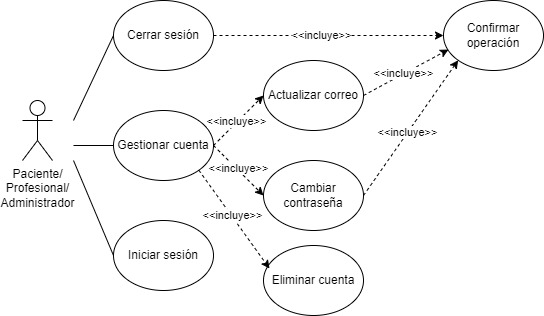
\includegraphics[width=1\textwidth]{img/CUdiagramas/CU-todos.jpg}
    \caption{CU-Administradores, Pacientes y Profesionales}
    \label{fig:CU-todos}
\end{figure}

\begin{figure}[h]
    \centering
    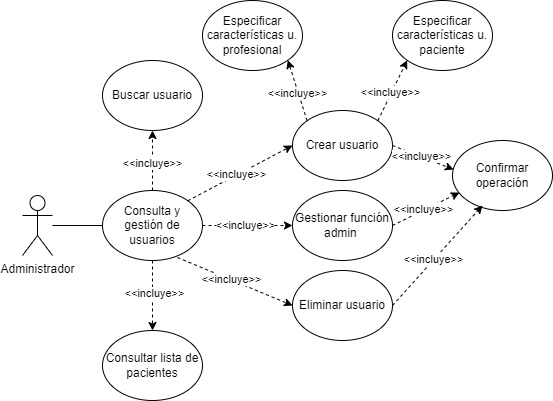
\includegraphics[width=1\textwidth]{img/CUdiagramas/CU-Administrador.jpg}
    \caption{CU-Administrador}
    \label{fig:CU-Administrador}
\end{figure}

\begin{figure}[h]
    \centering
    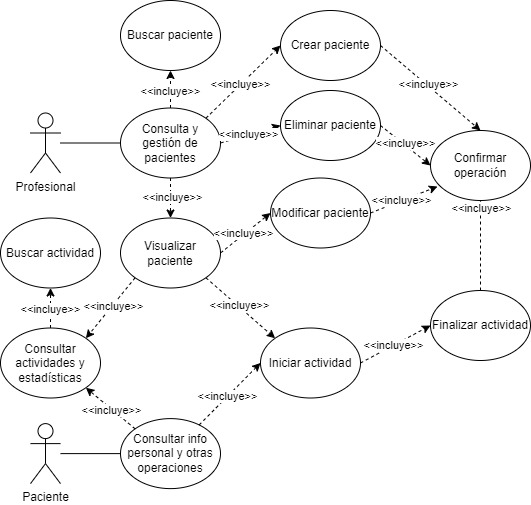
\includegraphics[width=1\textwidth]{img/CUdiagramas/CU-Paciente_Profesional.jpg}
    \caption{CU-Pacientes y Profesionales}
    \label{fig:CU-Paciente_Profesional}
\end{figure}


\section{Explicación Casos de Uso.}
Las tablas de explicación de Casos de Uso permiten proporcionar información detallada y organizada relativa a las funcionalidades del sistema y su integración. Facilitan el manejo de excepciones y sirven de guía para el posterior procceso de desarrollo, evitando errores que podrían tener importantes repercusiones en el avance del proyecto.  

% Caso de Uso 1 -> Iniciar sesión. -> ACABADO
\begin{table}[p]
	\centering
	\begin{tabularx}{\linewidth}{ p{0.21\columnwidth} p{0.71\columnwidth} }
		\toprule
		\textbf{CU-1}    & \textbf{Iniciar sesión}\\
		\toprule
        \textbf{Versión}              & 1.0    \\
		\textbf{Autor}                & Inés Martos Barbero \\
		\textbf{Requisitos asociados} & RF-01 \\
		\textbf{Descripción}          & Acceso del usuario al sistema mediante la selección del tipo de usuario y la autenticación de correo electrónico y contraseña. \\
		\textbf{Precondición}         & El usuario debe estar dado de alta en el sistema. \\
		\textbf{Acciones}             &
		\begin{enumerate}
			\def\labelenumi{\arabic{enumi}.}
			\tightlist
			\item Seleccionar tipo de usuario: paciente/profesional/administrador
			\item Ingresar credenciales (correo electrónico y contraseña)
            \item Validar credenciales
		\end{enumerate}\\
		\textbf{Postcondiciones}        & 
        \begin{enumerate}
			\def\labelenumi{\arabic{enumi}.}
			\tightlist
			\item Acceso al sistema concedido
			\item Inicio de sesión registrado para propósitos de seguimiento y seguridad
		\end{enumerate}\\
		\textbf{Excepciones}          & 
        \begin{enumerate}
			\def\labelenumi{\arabic{enumi}.}
			\tightlist
            \item Tipo de usuario no seleccionado. Alerta indicando que es necesaria la selección
            \item Ausencia de credenciales. El sistema pide que se completen los campos de correo electrónico y contraseña
			\item Credenciales incorrectas. Mensaje de aviso y permitir hasta 3 nuevos intentos
			\item Múltiples intentos fallidos. La cuenta será bloqueada un total de 5 minutos por seguridad
		\end{enumerate}\\
		\textbf{Importancia}          & Alta \\
		\bottomrule
	\end{tabularx}
	\caption{CU-1 Iniciar sesión}
    \label{CU-1}
\end{table}

% Caso de Uso 2 -> Confirmar operación. -> ACABADO
\begin{table}[p]
	\centering
	\begin{tabularx}{\linewidth}{ p{0.21\columnwidth} p{0.71\columnwidth} }
		\toprule
		\textbf{CU-2}    & \textbf{Confirmar operación}\\
		\toprule
        \textbf{Versión}              & 1.0    \\
		\textbf{Autor}                & Inés Martos Barbero \\
		\textbf{Requisitos asociados} & RF-03, RF-04, RF-07, RF-08 \\
		\textbf{Descripción}          & Verificación y aprobación de acciones críticas o cambios significativos en el sistema. \\
		\textbf{Precondición}         & Operación pendiente de confirmación \\
		\textbf{Acciones}             &
		\begin{enumerate}
			\def\labelenumi{\arabic{enumi}.}
			\tightlist
			\item El sistema muestra al usuario una ventana emergente para que este confirme la operación
			\item Confirmación o rechazo de la operación a través de un clic
		\end{enumerate}\\
		\textbf{Postcondición}        & Operación confirmada y llevada a cabo \\
        \textbf{Excepción}            & Operación cancelada. El sistema devuelve al usuario a la pantalla anterior sin realizar el cambio que se iba a llevar a cabo \\
		\textbf{Importancia}          & Media \\
		\bottomrule
	\end{tabularx}
	\caption{CU-2 Confirmar operación}
    \label{CU-2}
\end{table}

% Caso de Uso 3 -> Gestionar cuenta. -> ACABADO
\begin{table}[p]
	\centering
	\begin{tabularx}{\linewidth}{ p{0.21\columnwidth} p{0.71\columnwidth} }
		\toprule
		\textbf{CU-3}    & \textbf{Gestionar cuenta}\\
		\toprule
		\textbf{Versión}              & 1.0    \\
		\textbf{Autor}                & Inés Martos Barbero \\
		\textbf{Requisitos asociados} & RF-07 \\
		\textbf{Descripción}          & Administración de las credenciales del usuario necesarias para el inicio de sesión \\
		\textbf{Precondición}         & Usuario autenticado \\
		\textbf{Acciones}             &
		\begin{enumerate}
			\def\labelenumi{\arabic{enumi}.}
			\tightlist
			\item Acceso a la ventana de gestión de la cuenta y presentación de las opciones que esta ofrece
			\item Selección de la operación que se quiere realizar; CU-4 Actualizar correo, CU-5 Cambiar contraseña
		\end{enumerate}\\ 
		\textbf{Postcondiciones}        &
		\begin{enumerate}
			\def\labelenumi{\arabic{enumi}.}
			\tightlist
			\item Visualización de la información de la cuenta y las opciones disponibles.
			\item Redirección a casos de uso específicos
		\end{enumerate}\\
		\textbf{Excepción}          & El usuario puede decidir no realizar ninguna de las operaciones y regresar a la pantalla anterior, página de inicio o cualquiera de las opciones del menú principal \\
		\textbf{Importancia}          & Media \\
		\bottomrule
	\end{tabularx}
	\caption{CU-3 Gestionar cuenta}
     \label{CU-3}
\end{table}


% Caso de Uso 4 -> Actualizar correo. -> ACABADO
\begin{table}[p]
	\centering
	\begin{tabularx}{\linewidth}{ p{0.21\columnwidth} p{0.71\columnwidth} }
		\toprule
		\textbf{CU-4}    & \textbf{Actualizar correo}\\
		\toprule
		\textbf{Versión}              & 1.0    \\
		\textbf{Autor}                & Inés Martos Barbero \\
		\textbf{Requisitos asociados} & RF-07 \\
		\textbf{Descripción}          & Cambio del correo electrónico asociado a la cuenta del usuario \\
		\textbf{Precondición}         & Redirección desde 'Gestionar Cuenta' CU-3 \\
		\textbf{Acciones}             &
		\begin{enumerate}
			\def\labelenumi{\arabic{enumi}.}
			\tightlist
			\item Introducir la nueva dirección de correo en el campo correspondiente
			\item Verificación del nuevo correo introducido. El sistema solicita al usuario que reingrese el correo para confirmar que es el correcto.
                \item Seleccionar de la opción 'aplicar cambios'
                \item Confirmación de la operación, CU-2
		\end{enumerate}\\
		\textbf{Postcondiciones}        &
		\begin{enumerate}
			\def\labelenumi{\arabic{enumi}.}
			\tightlist
			\item Actualización del correo electrónico y notificación de operación exitosa
                \item Redirección a la ventana de Gestión de la cuenta (CU-2, CU-3)
		\end{enumerate}\\
		\textbf{Excepciones}          & 
            \begin{enumerate}
			\def\labelenumi{\arabic{enumi}.}
			\tightlist
			\item Campo vacío. Solicitar al usuario que introduzca la dirección de correo en los dos campos habilitados para ello
                \item Error de verificación: los correos introducidos no coinciden. Situación comunicada al usuario para que este actúe en consecuencia
                \item Formato de correo electrónico no válido. El sistema informa al usuario, solicita modificación y no se permite el cambio
                \item Correo electrónico en uso. La dirección de correo introducida ya se encuentra asociada a otra cuenta. Se informa del problema al usuario y no se permite el cambio
                \item Botón 'Cancelar operación' redirecciona a la pantalla de 'Gestión de la cuenta'
		\end{enumerate}\\
		\textbf{Importancia}          & Baja \\
		\bottomrule
	\end{tabularx}
	\caption{CU-4 Actualizar correo}
    \label{CU-4}
\end{table}

% Caso de Uso 5 -> Cambiar contraseña. -> ACABADO
\begin{table}[p]
	\centering
	\begin{tabularx}{\linewidth}{ p{0.21\columnwidth} p{0.71\columnwidth} }
		\toprule
		\textbf{CU-5}    & \textbf{Cambiar contraseña}\\
		\toprule
		\textbf{Versión}              & 1.0    \\
		\textbf{Autor}                & Inés Martos Barbero \\
		\textbf{Requisitos asociados} & RF-07 \\
		\textbf{Descripción}          & Modificación de la contraseña actual del usuario \\
		\textbf{Precondición}         & Redirección desde 'Gestionar Cuenta' CU-3 \\
		\textbf{Acciones}             &
		\begin{enumerate}
			\def\labelenumi{\arabic{enumi}.}
			\tightlist
			\item Ingresar la contraseña actual para verificar la identidad del usuario
                \item Introducir nueva contraseña en el campo correspondiente
                \item Repetir contraseña
			\item Seleccionar de la opción 'aplicar cambios'
                \item Confirmación de la operación, CU-2
		\end{enumerate}\\
		\textbf{Postcondiciones}        &
		\begin{enumerate}
			\def\labelenumi{\arabic{enumi}.}
			\tightlist
			\item Actualización de la contraseña y notificación de operación exitosa
                \item Redirección a la ventana de Gestión de la cuenta (CU-2, CU-3)
		\end{enumerate}\\
		\textbf{Excepciones}          & 
            \begin{enumerate}
			\def\labelenumi{\arabic{enumi}.}
			\tightlist
			\item Campo vacío. Solicitar al usuario que rellene todos los campos
                \item Contraseña actual incorrecta. Notificación al usuario y solicitud para que se vuelva a introducir
                \item Error de verificación. Las nuevas contraseñas introducidas no coinciden entre sí. Se informa al usuario y se solicita modificación
                \item Botón 'Cancelar operación' redirecciona a la pantalla de 'Gestión de la cuenta'
		\end{enumerate}\\
		\textbf{Importancia}          & Baja \\
		\bottomrule
	\end{tabularx}
	\caption{CU-5 Cambiar contraseña}
    \label{CU-5}
\end{table}

% Caso de Uso 6 -> Cerrar sesión. -> ACABADO
\begin{table}[p]
	\centering
	\begin{tabularx}{\linewidth}{ p{0.21\columnwidth} p{0.71\columnwidth} }
		\toprule
		\textbf{CU-6}    & \textbf{Cerrar sesión}\\
		\toprule
		\textbf{Versión}              & 1.0    \\
		\textbf{Autor}                & Inés Martos Barbero \\
		\textbf{Requisitos asociados} & RF-08 \\
		\textbf{Descripción}          & Desconexión segura del usuario del sistema \\
		\textbf{Precondición}         & Usuario autenticado (sesión iniciada) \\
		\textbf{Acciones}             &
		\begin{enumerate}
			\def\labelenumi{\arabic{enumi}.}
			\tightlist
			\item Selección de 'Cerrar Sesión' desde la opción del menú principal
			\item Confirmar operación, CU-2
		\end{enumerate}\\
		\textbf{Postcondiciones}        & 
            \begin{enumerate}
			\def\labelenumi{\arabic{enumi}.}
			\tightlist
			\item Sesión Cerrada
			\item Redirección a la pantalla de inicio de sesión (CU-1)
		\end{enumerate}\\
		\textbf{Excepción}          & Operación cancelada desde CU-2  \\
		\textbf{Importancia}          & Alta  \\
		\bottomrule
	\end{tabularx}
	\caption{CU-6 Cerrar sesión.}
    \label{CU-6}
\end{table}

% Caso de Uso 7 -> Consulta y gestión de usuarios. -> ACABADO
\begin{table}[p]
	\centering
	\begin{tabularx}{\linewidth}{ p{0.21\columnwidth} p{0.71\columnwidth} }
		\toprule
		\textbf{CU-7}    & \textbf{Consulta y gestión de usuarios}\\
		\toprule
		\textbf{Versión}              & 1.1    \\
		\textbf{Autor}                & Inés Martos Barbero \\
		\textbf{Requisitos asociados} & RF-02, RF-03 \\
		\textbf{Descripción}          & Revisión y manejo de los perfiles de usuarios registrados en el sistema \\
		\textbf{Precondición}         & Usuario con permisos administrativos accede a su pantalla de inicio \\
		\textbf{Acciones}             &
		\begin{enumerate}
			\def\labelenumi{\arabic{enumi}.}
			\tightlist
			\item Visualizar todos los datos, diferentes para cada tipo de usuario
			\item A través de una barra de búsqueda se puede realizar un filtrado de usuarios: CU-8 Buscar usuario
            \item Presionar el botón 'Nuevo usuario' para acceder a CU-9 Crear usuario
            \item Existen 2 botones diferentes para usuarios de tipo profesional que permiten controlar sus funciones de administrador a través de CU-12 Gestionar función admin de usuario profesional
            \item Hacer click sobre el icono de la papelera: CU-13 Eliminar usuario
		\end{enumerate}\\
        \textbf{Postcondiciones}         & 
            \begin{enumerate}
			\def\labelenumi{\arabic{enumi}.}
			\tightlist
			\item Redirección a alguno de los CU mencionados
			\item Actualización de la base de datos de usuarios según la acción realizada
		\end{enumerate}\\
		\textbf{Excepción}          & Fallos en alguno de los casos de uso que comprende \\
		\textbf{Importancia}          & Alta \\
		\bottomrule
	\end{tabularx}
	\caption{CU-7 Consulta y gestión de usuarios}
    \label{CU-7}
\end{table}

% Caso de Uso 8 -> Buscar usuario.  -> ACABADO
\begin{table}[p]
	\centering
	\begin{tabularx}{\linewidth}{ p{0.21\columnwidth} p{0.71\columnwidth} }
		\toprule
		\textbf{CU-8}    & \textbf{Buscar usuario}\\
		\toprule
		\textbf{Versión}              & 1.1    \\
		\textbf{Autor}                & Inés Martos Barbero \\
		\textbf{Requisitos asociados} & RF-02 \\
		\textbf{Descripción}          & Localización de usuarios dentro del sistema a través de nombre, apellidos, email y tipo de usuario \\
		\textbf{Precondiciones}         & 
            \begin{enumerate}
			\def\labelenumi{\arabic{enumi}.}
			\tightlist
			\item Usuario de tipo administrador autenticado
			\item Acceso desde la pantalla de inicio
		\end{enumerate}\\
		\textbf{Acciones}             &
		\begin{enumerate}
			\def\labelenumi{\arabic{enumi}.}
			\tightlist
			\item Ingreso manual de los criterios de búsqueda: nombre, apellidos, correo electrónico o tipo de usuario
			\item Envío de la solicitud de búsqueda. Botón lupa o 'buscar' para la obtención de los resultados
		\end{enumerate}\\
		\textbf{Postcondiciones}        & 
            \begin{enumerate}
			\def\labelenumi{\arabic{enumi}.}
			\tightlist
			\item Presentación de una lista de usuarios que cumplen con los criterios de búsqueda. Se muestra su nombre, apellidos, correo y rol.
			\item Se siguen ofreciendo opciones de gestión de usuarios: CU-9, CU-12, CU-13, CU-14
            \item Opción de eliminar el filtro aplicado y volver a mostrar todos los usuarios. Botón 'Retroceder en la búsqueda'
		\end{enumerate}\\
		\textbf{Excepciones}          & 
            \begin{enumerate}
			\def\labelenumi{\arabic{enumi}.}
			\tightlist
			\item Búsqueda sin resultados
			\item Formato erróneo del correo electrónico introducido
            \item Error en la escritura del tipo de usuario
		\end{enumerate}\\
		\textbf{Importancia}          & Media \\
		\bottomrule
	\end{tabularx}
	\caption{CU-8 Buscar usuario}
    \label{CU-8}
\end{table}

% Caso de Uso 9 -> Crear usuario   -> ACABADO
\begin{table}[p]
	\centering
	\begin{tabularx}{\linewidth}{ p{0.21\columnwidth} p{0.71\columnwidth} }
		\toprule
		\textbf{CU-9}    & \textbf{Crear usuario}\\
		\toprule
		\textbf{Versión}              & 1.0    \\
		\textbf{Autor}                & Inés Martos Barbero \\
		\textbf{Requisitos asociados} & RF-03 \\
		\textbf{Descripción}          & Registro de un nuevo usuario en el sistema, ya sea paciente, profesional o administrador \\
		\textbf{Precondición}         & Usuario administrador clica sobre 'Nuevo usuario' \\
		\textbf{Acciones}             &
		\begin{enumerate}
			\def\labelenumi{\arabic{enumi}.}
			\tightlist
			\item Completar los campos obligatorios de 'Nombre' y 'Apellidos'.
            \item Introducir obligatoriamente el correo electrónico. Es necesario repetirlo para evitar fallos de escritura
            \item Introducir contraseña para el acceso del usuario que se está creando. Hay que repetirla para evitar fallos de escritura. Recomendación: introducir el año de nacimiento y que el propio usuario la cambie con posterioridad
            \item Seleccionar tipo de usuario: profesional (CU-10), paciente (CU-11) o administrador
            \item Clicar en 'Guardar cambios' para continuar el proceso de creación
            \item Cancelar la creación del nuevo usuario seleccionando el botón 'Descartar cambios'
            \item Redireccionamiento a CU-2
		\end{enumerate}\\
		\textbf{Postcondiciones}        & 
            \begin{enumerate}
    			\def\labelenumi{\arabic{enumi}.}
    			\tightlist
    			\item Usuario registrado en el sistema 
                \item Notificación de la creación exitosa del usuario
    		\end{enumerate}\\
		\textbf{Excepciones}          & 
            \begin{enumerate}
    			\def\labelenumi{\arabic{enumi}.}
    			\tightlist
    			\item Selección de un único tipo de usuario 
                \item Datos incompletos. Solicitud para que se completen todos los campos 
                \item Error formato de email no adecuado
                \item Datos incorrectos. La información en los campos email/contraseña no coincide entre sí
                \item Conflicto de datos. Ya existe un usuario con mismo nombre y apellidos y/o correo electrónico
    		\end{enumerate}\\
		\textbf{Importancia}          & Alta \\
		\bottomrule
	\end{tabularx}
	\caption{CU-9 Crear usuario}
    \label{CU-9}
\end{table}

% Caso de Uso 10 -> Especificar características usuario profesional
\begin{table}[p]
	\centering
	\begin{tabularx}{\linewidth}{ p{0.21\columnwidth} p{0.71\columnwidth} }
		\toprule
		\textbf{CU-10}    & \textbf{Especificar características usuario profesional}\\
		\toprule
		\textbf{Versión}              & 1.0    \\
		\textbf{Autor}                & Inés Martos Barbero \\
		\textbf{Requisitos asociados} & RF-03 \\
		\textbf{Descripción}          & Define las características específicas de los usuarios profesionales \\
		\textbf{Precondiciones}         & 
            \begin{enumerate}
    			\def\labelenumi{\arabic{enumi}.}
    			\tightlist
    			\item Usuario administrador
    			\item En el proceso de creación de nuevo usuario (CU-9) se ha seleccionado el tipo de usuario como 'profesional'
    		\end{enumerate}\\
		\textbf{Acciones}             &
    		\begin{enumerate}
    			\def\labelenumi{\arabic{enumi}.}
    			\tightlist
    			\item Seleccionar la casilla 'proporcionar rol administrador' si se le quieren conceder dichos permisos
    			\item Escoger el método de asignación de pacientes.Para la selección manual se desplegarán todos los pacientes y también se podrá buscar por nombre y/o apellidos
    		\end{enumerate}\\
		\textbf{Postcondición}        & Los detalles quedan asociados al nuevo perfil \\
		\textbf{Excepciones}          & 
            \begin{enumerate}
    			\def\labelenumi{\arabic{enumi}.}
    			\tightlist
    			\item Método de selección de pacientes no indicado
    			\item Selección de pacientes manual no realizada. En caso de que esta sea la opción escogida
    		\end{enumerate}\\
		\textbf{Importancia}          & Alta\\
		\bottomrule
	\end{tabularx}
	\caption{CU-10 Especificar características usuario profesional}
    \label{CU-10}
\end{table}

% Caso de Uso 11 -> Especificar características usuario paciente
\begin{table}[p]
	\centering
	\begin{tabularx}{\linewidth}{ p{0.21\columnwidth} p{0.71\columnwidth} }
		\toprule
		\textbf{CU-11}    & \textbf{Especificar características usuario paciente}\\
		\toprule
		\textbf{Versión}              & 1.0    \\
		\textbf{Autor}                & Inés Martos Barbero \\
		\textbf{Requisitos asociados} & RF-03 \\
		\textbf{Descripción}          & Define las características específicas de los pacientes \\
		\textbf{Precondiciones}         & 
            \begin{enumerate}
    			\def\labelenumi{\arabic{enumi}.}
    			\tightlist
    			\item Usuario administrador
    			\item En el proceso de creación de nuevo usuario (CU-9) se ha seleccionado el tipo de usuario como 'paciente'
    		\end{enumerate}\\
		\textbf{Acciones}             &
		\begin{enumerate}
			\def\labelenumi{\arabic{enumi}.}
			\tightlist
			\item Completar campos 'altura' y 'sexo'
			\item Selección del método de asignación de profesional. La forma manual despliega una lista en la que también se puede buscar por nombre y/o apellidos
		\end{enumerate}\\
        \textbf{Postcondición}        & Los detalles quedan asociados al nuevo perfil \\
        \textbf{Excepciones}          & 
            \begin{enumerate}
    			\def\labelenumi{\arabic{enumi}.}
    			\tightlist
    			\item Información incompleta. Falta rellenar el campo altura y/o sexo, lo que se solicitará a través de una notificación
                \item Formato erróneo. El formato en el que se ha introducido la información del campo altura y/o sexo es erróneo
                \item Método de asignación de profesional no indicado
    			\item Selección de profesional manual no realizada. En caso de que esta sea la opción escogida
    		\end{enumerate}\\
		\textbf{Importancia}          & Alta \\
		\bottomrule
	\end{tabularx}
	\caption{CU-11 Especificar características usuario paciente}
    \label{CU-11}
\end{table}

% Caso de Uso 12 -> Gestionar función admin  -> ACABADO
\begin{table}[p]
	\centering
	\begin{tabularx}{\linewidth}{ p{0.21\columnwidth} p{0.71\columnwidth} }
		\toprule
		\textbf{CU-12}    & \textbf{Gestionar función admin}\\
		\toprule
		\textbf{Versión}              & 1.0    \\
		\textbf{Autor}                & Inés Martos Barbero \\
		\textbf{Requisitos asociados} & RF-03 \\
		\textbf{Descripción}          & Asignar o revocar roles administrativos a usuarios profesionales a través de un botón que indica el estado actual del rol \\
		\textbf{Precondiciones}         & 
            \begin{enumerate}
    			\def\labelenumi{\arabic{enumi}.}
    			\tightlist
    			\item Usuario administrador autenticado
    			\item El administrador debe estar visualizando el perfil de un usuario profesional en su pantalla de inicio
		  \end{enumerate}\\
		\textbf{Acciones}             &
		\begin{enumerate}
			\def\labelenumi{\arabic{enumi}.}
			\tightlist
			\item Identificar el profesional cuyo rol se desea gestionar
			\item Según el estado actual, el administrador selecciona el botón correspondiente: 'Hacer admin' para otorgar funciones administrativas, o 'Quitar admin' para revocarlas
            \item Tras presionar el botón se redirige a CU-2 para confirmar la operación
		\end{enumerate}\\
		\textbf{Postcondiciones}        & 
            \begin{enumerate}
    			\def\labelenumi{\arabic{enumi}.}
    			\tightlist
    			\item Actualización del perfil profesional reflejando la adición o eliminación de funciones administrativas
    			\item Notificación de actualización exitosa
		  \end{enumerate}\\
		\textbf{Excepciones}          & 
            \begin{enumerate}
    			\def\labelenumi{\arabic{enumi}.}
    			\tightlist
    			\item No se localiza el profesional que se quiere modificar
    			\item Operación cancelada en CU-2. No se realiza ningún cambio
		  \end{enumerate}\\
		\textbf{Importancia}          & Baja \\
		\bottomrule
	\end{tabularx}
	\caption{CU-12 Gestionar función admin}
    \label{CU-12}
\end{table}

% Caso de Uso 13 -> Eliminar usuario     -> ACABADO
\begin{table}[p]
	\centering
	\begin{tabularx}{\linewidth}{ p{0.21\columnwidth} p{0.71\columnwidth} }
		\toprule
		\textbf{CU-13}    & \textbf{Eliminar usuario}\\
		\toprule
		\textbf{Versión}              & 1.0    \\
		\textbf{Autor}                & Inés Martos Barbero \\
		\textbf{Requisitos asociados} & RF-03 \\
		\textbf{Descripción}          & Facilita la eliminación de usuarios del sistema \\
		\textbf{Precondición}         & El usuario administrador debe estar visualizando el usuario que pretende eliminar \\
		\textbf{Acciones}             &
		\begin{enumerate}
			\def\labelenumi{\arabic{enumi}.}
			\tightlist
			\item Hacer clic sobre el icono de papelera situado a la derecha de la información perteneciente al usuario de interés
			\item CU-2 para confirmación de la operación
		\end{enumerate}\\
		\textbf{Postcondición}        & Usuario seleccionado es eliminado del sistema. Si se trata de un paciente, desaparece de las listas de profesionales. Si se trata de un profesional, sus pacientes son redistribuidos automáticamente entre otros profesionales \\
		\textbf{Excepción}          & Operación CU-2 cancelada, el usuario no se elimina \\
		\textbf{Importancia}          & Baja \\
		\bottomrule
	\end{tabularx}
	\caption{CU-13 Eliminar usuario}
    \label{CU-13}
\end{table}

% Caso de Uso 14 -> Consultar lista de pacientes  -> ACABADO
\begin{table}[p]
	\centering
	\begin{tabularx}{\linewidth}{ p{0.21\columnwidth} p{0.71\columnwidth} }
		\toprule
		\textbf{CU-14}    & \textbf{Consultar lista de pacientes}\\
		\toprule
		\textbf{Versión}              & 1.0    \\
		\textbf{Autor}                & Inés Martos Barbero \\
		\textbf{Requisitos asociados} & RF-02, RF-03 \\
		\textbf{Descripción}          & Permite visualizar la lista completa de pacientes asociados a un profesional específico, y sus opciones de gestión \\
		\textbf{Precondición}         & Usuario administrador selecciona el botón 'listado de pacientes' correspondiente al profesional de interés, desde la pantalla de inicio (consulta y gestión de usuarios) \\
		\textbf{Acciones}             &
		\begin{enumerate}
			\def\labelenumi{\arabic{enumi}.}
			\tightlist
			\item El usuario presiona el botón 'listado de pacientes'
            \item Visualización de los pacientes asignados al profesional de interés. Incluye la siguiente información: nombre, apellidos, email y profesionales asignados
            \item Barra de búsqueda de paciente CU-21
			\item Ofrece la posibilidad de eliminar pacientes CU-13
            \item Botón con opción de volver a la pantalla de inicio
            \item Botón para realizar una redistribución automática de pacientes si se considera que el profesional tiene demasiados a su cargo. Se repartirán pacientes a otros profesionales. Redirecciona a CU-2
		\end{enumerate}\\
		\textbf{Postcondiciones}        & 
        \begin{enumerate}
			\def\labelenumi{\arabic{enumi}.}
			\tightlist
			\item El administrador obtiene una visión completa de los pacientes asignados a un profesional específico
			\item Tras la redistribución automática se muestra la lista actualizada y se envía notificación de operación exitosa
		\end{enumerate}\\
		\textbf{Excepciones}          & 
        \begin{enumerate}
			\def\labelenumi{\arabic{enumi}.}
			\tightlist
			\item Paciente no localizado
			\item Redistribución automática no aprobada en CU-2
		\end{enumerate}\\
		\textbf{Importancia}          & Baja \\
		\bottomrule
	\end{tabularx}
	\caption{CU-14 Consultar lista de pacientes}
    \label{CU-14}
\end{table}

% Caso de Uso 15 -> Consultar información personal y otras operaciones    -> ACABADO
\begin{table}[p]
	\centering
	\begin{tabularx}{\linewidth}{ p{0.21\columnwidth} p{0.71\columnwidth} }
		\toprule
		\textbf{CU-15}    & \textbf{Consultar información personal y otras operaciones}\\
		\toprule
		\textbf{Versión}              & 1.0    \\
		\textbf{Autor}                & Inés Martos Barbero \\
		\textbf{Requisitos asociados} & RF-02, RF-03, RF-04, RF-05, RF-06 \\
		\textbf{Descripción}          & Permite a los usuarios acceder a su información personal y a las funciones principales de su cuenta \\
		\textbf{Precondición}         & Paciente accede a su cuenta \\
		\textbf{Acciones}             &
		\begin{enumerate}
			\def\labelenumi{\arabic{enumi}.}
			\tightlist
			\item Visualización de la información personal relativa al paciente que ha iniciado sesión: sexo, altura, email y profesionales a cargo de su tratamiento
			\item Las opciones que se presentan en forma de botones son: 'iniciar actividad' (CU-16), 'actividades y estadísticas' (CU-18) y 'actividad offline'.
            \item Escoger la opción que se desea realizar
            \item 'actividad offline' mostrará una pestaña informando al usuario de cómo usar el dispositivo físico para realizar una actividad sin necesidad de conexión a la página web
		\end{enumerate}\\
		\textbf{Postcondición}        & Visualización de la información y, en caso de pinchar uno de los botones, redirección a una pestaña nueva \\
		\textbf{Excepción}          & Tras acceder a alguna de las opciones se podrá regresar a la pantalla de inicio en cualquier momento sin realizar cambios \\
		\textbf{Importancia}          & Alta \\
		\bottomrule
	\end{tabularx}
	\caption{CU-15 Consultar información personal y otras operaciones}
    \label{CU-15}
\end{table}

% Caso de Uso 16 -> Iniciar actividad    -> ACABADO
\begin{table}[p]
	\centering
	\begin{tabularx}{\linewidth}{ p{0.21\columnwidth} p{0.71\columnwidth} }
		\toprule
		\textbf{CU-16}    & \textbf{Iniciar actividad}\\
		\toprule
		\textbf{Versión}              & 1.0    \\
		\textbf{Autor}                & Inés Martos Barbero \\
		\textbf{Requisitos asociados} & RF-04 \\
		\textbf{Descripción}          & Comenzar a visualizar en tiempo real y a registrar los datos de una actividad del paciente \\
		\textbf{Precondición}         & Usuario profesional o paciente acceden a la opción 'Iniciar actividad' \\
		\textbf{Acciones}             &
		\begin{enumerate}
			\def\labelenumi{\arabic{enumi}.}
			\tightlist
			\item El usuario presióna el botón 'Iniciar actividad'
			\item Redirección a CU-2 para confirmar la operación
            \item Una nueva página muestra en tiempo real los datos de la actividad: distancia recorrida, velocidad, número de pasos y número de bloqueos
            \item Opción 'Finalizar actividad' (CU-17) para concluir el registro de datos
		\end{enumerate}\\
		\textbf{Postcondición}        & Visualizar en tiempo real los datos de la actividad \\
		\textbf{Excepciones}          & 
        \begin{enumerate}
			\def\labelenumi{\arabic{enumi}.}
			\tightlist
			\item CU-2 cancela la operación
			\item Problemas de conectividad que no permiten la visualización en tiempo real
		\end{enumerate}\\
		\textbf{Importancia}          & Alta \\
		\bottomrule
	\end{tabularx}
	\caption{CU-16 Iniciar actividad}
    \label{CU-16}
\end{table}

% Caso de Uso 17 -> Finalizar actividad    -> ACABADO
\begin{table}[p]
	\centering
	\begin{tabularx}{\linewidth}{ p{0.21\columnwidth} p{0.71\columnwidth} }
		\toprule
		\textbf{CU-17}    & \textbf{Finalizar actividad}\\
		\toprule
		\textbf{Versión}              & 1.0    \\
		\textbf{Autor}                & Inés Martos Barbero \\
		\textbf{Requisitos asociados} & RF-04 \\
		\textbf{Descripción}          & Concluir el registro de datos de una actividad en proceso \\
		\textbf{Precondición}         & Que una actividad se esté llevando a cabo y el botón 'Finalizar actividad' esté disponible \\
		\textbf{Acciones}             &
		\begin{enumerate}
			\def\labelenumi{\arabic{enumi}.}
			\tightlist
			\item Presionar el botón 'Finalizar actividad'
			\item Confirmar operación CU-2
            \item Seleccionar opción para la finalización: 'Descartar actividad' si no se quieren almacenar los datos, o 'Guardar actividad' si se quieren guardar los datos para consultas futuras
		\end{enumerate}\\
		\textbf{Postcondiciones}        & 
        \begin{enumerate}
			\def\labelenumi{\arabic{enumi}.}
			\tightlist
			\item Actividad finalizada y almacenada para su posterior consulta
			\item Se muestra la pantalla con los datos personales del paciente
		\end{enumerate}\\
		\textbf{Excepciones}          & 
        \begin{enumerate}
			\def\labelenumi{\arabic{enumi}.}
			\tightlist
			\item CU-2 Cancela la operación
			\item No se almacenan los datos de la actividad
		\end{enumerate}\\
		\textbf{Importancia}          & Alta  \\
		\bottomrule
	\end{tabularx}
	\caption{CU-17 Finalizar actividad}
    \label{CU-17}
\end{table}

% Caso de Uso 18 -> Consultar actividades y estadísticas    -> ACABADO
\begin{table}[p]
	\centering
	\begin{tabularx}{\linewidth}{ p{0.21\columnwidth} p{0.71\columnwidth} }
		\toprule
		\textbf{CU-18}    & \textbf{Consultar actividades y estadísticas}\\
		\toprule
		\textbf{Versión}              & 1.0    \\
		\textbf{Autor}                & Inés Martos Barbero \\
		\textbf{Requisitos asociados} & RF-05, RF-06 \\
		\textbf{Descripción}          & Permite acceder al listado de todas las actividades, consultarlas en un calendario y ver las estadísticas globales \\
		\textbf{Precondición}         & Acceso presionando el botón 'Actividades y estadísticas' desde la pantalla en la que se visualiza la información personal del paciente \\
		\textbf{Acciones}             &
		\begin{enumerate}
			\def\labelenumi{\arabic{enumi}.}
			\tightlist
			\item Visualizar todos los datos diferentes para cada actividad: ID, fecha, hora, número de bloqueos, distancia, velocidad media y número de pasos
            \item A través de una barra de búsqueda se puede realizar un filtrado de actividades: CU-19 Buscar actividad
            \item Apartado de estadísticas globales: media de bloqueos, distancia total, media de velocidades y media de pasos
			\item Calendario de actividades. Cada día almacena el nombre de la actividad realizada (ID): seleccionar una actividad muestra sus datos en una ventana emergente
		\end{enumerate}\\
		\textbf{Postcondición}        &  Visualización de actividades desde diferentes perspectivas\\
		\textbf{Excepción}          & No existencia de actividades almacenadas \\
		\textbf{Importancia}          & Alta  \\
		\bottomrule
	\end{tabularx}
	\caption{CU-18 Consultar actividades y estadísticas}
    \label{CU-18}
\end{table}

% Caso de Uso 19 -> Buscar actividad    -> ACABADO
\begin{table}[p]
	\centering
	\begin{tabularx}{\linewidth}{ p{0.21\columnwidth} p{0.71\columnwidth} }
		\toprule
		\textbf{CU-19}    & \textbf{Buscar actividad}\\
		\toprule
		\textbf{Versión}              & 1.0    \\
		\textbf{Autor}                & Inés Martos Barbero \\
		\textbf{Requisitos asociados} & RF-05, RF-06 \\
		\textbf{Descripción}          & Localización de actividades a través de ID, fecha, hora o número de bloqueos \\
		\textbf{Precondición}         & Usuario situado en la ventana de consulta de actividades y estadísticas \\
		\textbf{Acciones}             &
		\begin{enumerate}
			\def\labelenumi{\arabic{enumi}.}
			\tightlist
			\item Ingreso manual de los criterios de búsqueda: ID actividad, fecha, hora o número de bloqueos
			\item Envío de la solicitud de búsqueda. Botón lupa o 'buscar' para la obtención de resultados
		\end{enumerate}\\
		\textbf{Postcondiciones}        & 
        \begin{enumerate}
			\def\labelenumi{\arabic{enumi}.}
			\tightlist
			\item Presentación de una lista de actividades que cumplen con los criterios de búsqueda
			\item Se siguen visualizando el resto de funcionalidades del apartado de consulta de actividades y estadísticas
            \item Opción de eliminar el filtro aplicado y volver a mostrar todas las actividades. Botón 'Retroceder en la búsqueda'
		\end{enumerate}\\
		\textbf{Excepciones}          & 
        \begin{enumerate}
			\def\labelenumi{\arabic{enumi}.}
			\tightlist
			\item Búsqueda sin resultados
			\item Formato erróneo de los datos introducidos. Salta una alerta indicando cuales pueden ser los posibles problemas
		\end{enumerate}\\
		\textbf{Importancia}          &  Baja \\
		\bottomrule
	\end{tabularx}
	\caption{CU-19 Buscar actividad}
    \label{CU-19}
\end{table}

% Caso de Uso 20 -> Consulta y gestión de pacientes    -> ACABADO
\begin{table}[p]
	\centering
	\begin{tabularx}{\linewidth}{ p{0.21\columnwidth} p{0.71\columnwidth} }
		\toprule
		\textbf{CU-20}    & \textbf{Consulta y gestión de pacientes}\\
		\toprule
		\textbf{Versión}              & 1.0    \\
		\textbf{Autor}                & Inés Martos Barbero \\
		\textbf{Requisitos asociados} & RF-02, RF-03 \\
		\textbf{Descripción}          & Revisión y manejo de los perfiles de pacientes registrados en el sistema \\
		\textbf{Precondición}         & Usuario profesional autenticado accede a su pantalla de inicio \\
		\textbf{Acciones}             &
		\begin{enumerate}
			\def\labelenumi{\arabic{enumi}.}
			\tightlist
			\item Mostrar todos los datos, diferentes para cada paciente
			\item A través de una barra de búsqueda se puede realizar un filtrado de pacientes: CU-21 Buscar paciente
            \item Opción 'Consultar paciente' para visualizar sus datos personales y acceder a estadísticas, consulta y realización de actividades (CU-25)
            \item Presionar el botón 'Dar de alta paciente' para acceder a CU-22
            \item Hacer click sobre el icono de la papelera: CU-24 Eliminar usuario
		\end{enumerate}\\
		\textbf{Postcondiciones}        & 
        \begin{enumerate}
			\def\labelenumi{\arabic{enumi}.}
			\tightlist
			\item Visualición de todos los pacientes, sus datos y opciones de gestión
			\item Redirección a alguno de los CU mencionados
		\end{enumerate}\\
		\textbf{Excepción}          & Inexistencia de pacientes asignados al profesional que accede la plataforma \\
		\textbf{Importancia}          & Media \\
		\bottomrule
	\end{tabularx}
	\caption{CU-20 Consulta y gestión de pacientes}
    \label{CU-20}
\end{table}

% Caso de Uso 21 -> Buscar paciente    -> ACABADO
\begin{table}[p]
	\centering
	\begin{tabularx}{\linewidth}{ p{0.21\columnwidth} p{0.71\columnwidth} }
		\toprule
		\textbf{CU-21}    & \textbf{Buscar paciente}\\
		\toprule
		\textbf{Versión}              & 1.0    \\
		\textbf{Autor}                & Inés Martos Barbero \\
		\textbf{Requisitos asociados} & RF-02, RF-03 \\
		\textbf{Descripción}          & Localización de pacientes asignados a un profesional, a través de: nombre, apellidos o email \\
		\textbf{Precondición}         & Usuario profesional autenticado accede a su pantalla de inicio (consulta y gestión de pacientes) \\
		\textbf{Acciones}             &
		\begin{enumerate}
			\def\labelenumi{\arabic{enumi}.}
			\tightlist
			\item Ingreso manual de los criterios de búsqueda: nombre, apellidos o email
			\item Envío de la solicitud de búsqueda. Botón lupa o 'buscar' para la obtención de los resultados
		\end{enumerate}\\
		\textbf{Postcondiciones}        & 
        \begin{enumerate}
			\def\labelenumi{\arabic{enumi}.}
			\tightlist
			\item Presentación de una lista de pacientes que cumplen con los criterios de búsqueda
			\item Se siguen ofreciendo opciones de gestión de pacientes: CU-22, CU-24, CU-25
		\end{enumerate}\\
		\textbf{Excepciones}          & 
        \begin{enumerate}
			\def\labelenumi{\arabic{enumi}.}
			\tightlist
			\item Búsqueda sin resultados
			\item Formato erróneo del texto de búsqueda
		\end{enumerate}\\
		\textbf{Importancia}          & Baja \\
		\bottomrule
	\end{tabularx}
	\caption{CU-21 Buscar paciente}
    \label{CU-21}
\end{table}

% Caso de uso 22 -> Dar de alta paciente     -> ACABADO
\begin{table}[p]
	\centering
	\begin{tabularx}{\linewidth}{ p{0.21\columnwidth} p{0.71\columnwidth} }
		\toprule
		\textbf{CU-22}    & \textbf{Dar de alta paciente}\\
		\toprule
		\textbf{Versión}              & 1.0    \\
		\textbf{Autor}                & Inés Martos Barbero \\
		\textbf{Requisitos asociados} & RF-03 \\
		\textbf{Descripción}          & El profesional se auto-asigna un paciente \\
		\textbf{Precondición}         & Usuario profesional autenticado selecciona 'Dar de alta paciente' desde su pestaña de inicio (consulta y gestión de pacientes \\
		\textbf{Acciones}             &
		\begin{enumerate}
			\def\labelenumi{\arabic{enumi}.}
			\tightlist
			\item Acceder mediante el botón 'Dar de alta paciente'
			\item Seleccionar un paciente ya dado de alta en el sistema o crear un nuevo paciente (CU-23)
            \item Presionar botón 'Realizar operación' que redirigirá al profesional a CU-2
		\end{enumerate}\\
		\textbf{Postcondición}        & Paciente añadido al conjunto de pacientes del profesional que lo está dando de alta \\
		\textbf{Excepciones}          & 
        \begin{enumerate}
			\def\labelenumi{\arabic{enumi}.}
			\tightlist
			\item Botón 'Cancelar operación'
            \item CU-2 operación cancelada
		\end{enumerate}\\
		\textbf{Importancia}          & Media\\
		\bottomrule
	\end{tabularx}
	\caption{CU-22 Dar de alta paciente}
    \label{CU-22}
\end{table}

% Caso de Uso 23 -> Crear paciente     -> ACABADO
\begin{table}[p]
	\centering
	\begin{tabularx}{\linewidth}{ p{0.21\columnwidth} p{0.71\columnwidth} }
		\toprule
		\textbf{CU-23}    & \textbf{Crear paciente}\\
		\toprule
		\textbf{Versión}              & 1.0    \\
		\textbf{Autor}                & Inés Martos Barbero \\
		\textbf{Requisitos asociados} & RF-03 \\
		\textbf{Descripción}          & Profesional registra un nuevo usuario de tipo paciente en el sistema \\
		\textbf{Precondición}         & Usuario profesional autenticado que haya escogido la opción 'nuevo paciente' desde el apartado 'dar de alta paciente' \\
		\textbf{Acciones}             &
		\begin{enumerate}
			\def\labelenumi{\arabic{enumi}.}
			\tightlist
			\item Completar los campos obligatorios de nombre y apellidos
            \item Introducir obligatoriamente el correo electrónico. Es necesiario repetirlo para evitar fallos de escritura
            \item Introducir contraseña para el acceso del usuario que se está creando. Hay que repetirla para evitar fallos de escritura. Recomendación: introducir el año de nacimiento y que el propio usuario la cambie con posterioridad
			\item Rellenar campos altura y sexo.
            \item Asignación automática al profesional que está creando el usuario
		\end{enumerate}\\
		\textbf{Postcondiciones}        & 
        \begin{enumerate}
			\def\labelenumi{\arabic{enumi}.}
			\tightlist
			\item Usuario registrado en el sistema
            \item Notificación de creación exitosa
		\end{enumerate}\\
		\textbf{Excepciones}          & 
        \begin{enumerate}
			\def\labelenumi{\arabic{enumi}.}
			\tightlist
			\item Datos incompletos. Solicitud para que se completen todos los campos
            \item Error formato de email no adecuado
            \item Datos incorrectos. La información en los campos email/contraseña no coincide entre sí
            \item Conflicto de datos. Ya existe un usuario con mismo nombre y apellidos y/o correo electrónico
		\end{enumerate}\\
		\textbf{Importancia}          & Alta\\
		\bottomrule
	\end{tabularx}
	\caption{CU-23 Crear paciente}
    \label{CU-23}
\end{table}

% Caso de Uso 24 -> Eliminar paciente    -> ACABADO
\begin{table}[p]
	\centering
	\begin{tabularx}{\linewidth}{ p{0.21\columnwidth} p{0.71\columnwidth} }
		\toprule
		\textbf{CU-24}    & \textbf{Eliminar paciente}\\
		\toprule
		\textbf{Versión}              & 1.0    \\
		\textbf{Autor}                & Inés Martos Barbero \\
		\textbf{Requisitos asociados} & RF-03 \\
		\textbf{Descripción}          & Habilita la eliminación de un paciente de aquellos asignados al profesional que realiza la acción \\
		\textbf{Precondición}         & El usuario profesional debe estar visualizando el paciente que pretende eliminar \\
		\textbf{Acciones}             &
		\begin{enumerate}
			\def\labelenumi{\arabic{enumi}.}
			\tightlist
			\item Hacer clic sobre el icono de papelera situado a la derecha de la información perteneciente al usuario de interés
			\item CU-2 para confirmación de la operación
		\end{enumerate}\\
		\textbf{Postcondición}        & Paciente seleccionado es eliminado de la lista de pacientes del profesional que lo está eliminando. Si dicho paciente no está asignado a otros profesionales, se verá eliminado del sistema \\
		\textbf{Excepción}          & CU-2 operación cancelada, el paciente no se elimina \\
		\textbf{Importancia}          & Baja \\
		\bottomrule
	\end{tabularx}
	\caption{CU-24 Eliminar paciente}
    \label{CU-24}
\end{table}

% Caso de Uso 25 -> Visualizar paciente    -> ACABADO
\begin{table}[p]
	\centering
	\begin{tabularx}{\linewidth}{ p{0.21\columnwidth} p{0.71\columnwidth} }
		\toprule
		\textbf{CU-25}    & \textbf{Visualizar paciente}\\
		\toprule
		\textbf{Versión}              & 1.0    \\
		\textbf{Autor}                & Inés Martos Barbero \\
		\textbf{Requisitos asociados} & RF-02, RF-03, RF-04, RF-05, RF-06 \\
		\textbf{Descripción}          & Permite visualizar la información detallada de un paciente \\
		\textbf{Precondición}         & Profesional selecciona la opción 'visualizar paciente' del paciente de interés \\
		\textbf{Acciones}             &
		\begin{enumerate}
			\def\labelenumi{\arabic{enumi}.}
			\tightlist
			\item Mostrar la información personal del paciente seleccionado: sexo, altura, email y profesionales a cargo de su tratamiento
            \item Las opciones de gestión del paciente son: 'modificar datos' CU-26 y eliminar paciente (CU-24)
			\item Otras opciones son: 'iniciar actividad' (CU-16), 'actividades y estadísticas' (CU-18)
		\end{enumerate}\\
		\textbf{Postcondición}        & Visualización de la información y, en caso de pinchar uno de los botones, redirección a una pestaña nueva \\
		\textbf{Excepción}          & Tras acceder a alguna de las opciones se podrá regresar a la pantalla de visualización del paciente sin realizar cambios \\
		\textbf{Importancia}          & Alta \\
		\bottomrule
	\end{tabularx}
	\caption{CU-25 Visualizar paciente}
    \label{CU-25}
\end{table}

% Caso de Uso 26 -> Modificar paciente     -> ACABADO
\begin{table}[p]
	\centering
	\begin{tabularx}{\linewidth}{ p{0.21\columnwidth} p{0.71\columnwidth} }
		\toprule
		\textbf{CU-26}    & \textbf{Modificar paciente}\\
		\toprule
		\textbf{Versión}              & 1.0    \\
		\textbf{Autor}                & Inés Martos Barbero \\
		\textbf{Requisitos asociados} & RF-03 \\
		\textbf{Descripción}          & Actualización de los datos de un paciente \\
		\textbf{Precondición}         & Profesional selecciona la opción 'modificar paciente' desde la pantalla de visualización de dicho paciente \\
		\textbf{Acciones}             &
		\begin{enumerate}
			\def\labelenumi{\arabic{enumi}.}
			\tightlist
			\item Seleccionar 'modificar paciente' del paciente de interés
			\item Actualizar los datos que se considere necesario: nombre, apellidos, sexo, altura, email
            \item Presionar botón 'Aplicar cambios'
            \item Confirmar operación CU-2
		\end{enumerate}\\
		\textbf{Postcondición}        & Se aplican los cambios. Modificaciones visibles en la página de visualización de datos personales del paciente \\
		\textbf{Excepciones}          & CU-2 operación cancelada \\
		\textbf{Importancia}          & Alta o Media o Baja... \\
		\bottomrule
	\end{tabularx}
	\caption{CU-26 Modificar paciente}
    \label{CU-26}
\end{table}

% Caso de Uso 27 -> Eliminar cuenta    -> ACABADO
\begin{table}[p]
	\centering
	\begin{tabularx}{\linewidth}{ p{0.21\columnwidth} p{0.71\columnwidth} }
		\toprule
		\textbf{CU-27}    & \textbf{Eliminar cuenta}\\
		\toprule
		\textbf{Versión}              & 1.0    \\
		\textbf{Autor}                & Inés Martos Barbero \\
		\textbf{Requisitos asociados} & RF-07 \\
		\textbf{Descripción}          & Borrado de todos los datos del usuario que está ejecutando la acción \\
		\textbf{Precondición}         & Usuario registrado \\
		\textbf{Acciones}             &
		\begin{enumerate}
			\def\labelenumi{\arabic{enumi}.}
			\tightlist
			\item Seleccionar la opción 'eliminar cuenta' del menú
            \item Redireccionamiento a CU-2 
			\item Si el usuario eliminado es de tipo profesional, todos sus pacientes que no estén asignados a otros profesionales, se readjudicarán de forma automática
		\end{enumerate}\\
		\textbf{Postcondición}        & El usuario deja de existir por completo. Se elimina toda información relacionada \\
		\textbf{Excepciones}          & CU-2 operación cancelada \\
		\textbf{Importancia}          & Baja \\
		\bottomrule
	\end{tabularx}
	\caption{CU-27 Eliminar cuenta}
    \label{CU-27}
\end{table}


\section{Prototipos de interfaz.}
Una buena práctica antes de comenzar con la programación de la página web es la elaboración de wireframes sencillos, al menos, para las principales pestañas. Esto es esencial por varios motivos: 
\begin{itemize}
    \item Proporcionan mayor claridad y comprensión de los requisitos de la web, ayudando a guiar el desarrollo posterior.
    \item Permiten la detección temprana de problemas de usabilidad y otorgar importancia para la experiencia del usuario.
    \item Mejoran la comunicación entre las personas involucradas en el proceso de desarrollo (no aplicable a este proyecto).
\end{itemize}

En este caso, se han realizado wireframes para algunas de las ventanas más relevantes, mostrando una aproximación de lo que podría ser el resultado final.
\begin{itemize}
    \item Iniciar sesión. En la figura \ref{fig:Iniciar sesión} se muestran los campos a rellenar en la pantalla de acceso común a todos los usarios.
    \item Confirmar operación. La notificación \ref{fig:Confirmar operación} se mostrará ante operaciones delicadas como eliminación de pacientes para confirmar que el usuario realmente quiere llevar a cabo el proceso que ha iniciado (\ref{CU-2}).
    \item Consulta y gestión de usuarios. El menú de inicio del usuario administrador será similar a la figura \ref{fig:Consulta y gestión de usuarios} de la forma que indica CU-7 (\ref{CU-7}).
    \item Crear usuario. Frontend de CU-9 (\ref{CU-9}) representado en la figura \ref{fig:Crear usuario}. El administrador tendrá que rellenar los datos comunes a todos los usuarios y, posteriormente, según el tipo de usuario que esté dando de alta será neceario completar unos campos específicos.
    \item Consultar lista de pacientes. La Figura \ref{fig:Consultar lista de pacientes} es un primer boceto de la pantalla de inicio de un usuario profesional.
    \item Consultar información personal y otras operaciones. La pantalla de la Figura \ref{fig:Consultar info personal y otras actividades} es accesible tanto por pacientes (será su pantalla de inicio) como por profesionales cuando seleccionen el paciente que quieren visualizar.
    \item Iniciar actividad. Al seleccionar la función de iniciar actividad, CU-16 (\ref{CU-16}), el sistema se comunica con Arduino y este le enviará los datos en tiempo real a una interfaz como la de la Figura \ref{fig:Iniciar actividad}.
    \item Consultar actividades y estadísticas. Las imágenes de \ref{fig:Consultar actividades y estadísticas (Paciente)} y \ref{fig:Consultar actividades y estadísticas (Profesional)} reflejan la idea inicial de cómo organizar el CU-18 (\ref{CU-18}) para pacienes y profesionales respectivamente.
    \item Consulta y gestión de pacientes (\ref{fig:Consulta y gestión de pacientes}). Es la pantalla de inicio para profesionales.
    \item Crear paciente. Acción reservada a administradores mediante la cumplimentación del formulario \ref{fig:Crear paciente}. 
    \item Visualizar paciente. El profesional santiario tiene acceso a los datos de cada paciente estructurados como en la pestaña de la Figura \ref{fig:Visualizar paciente}.
\end{itemize}


% Iniciar sesión
\begin{figure}[h]
    \centering
    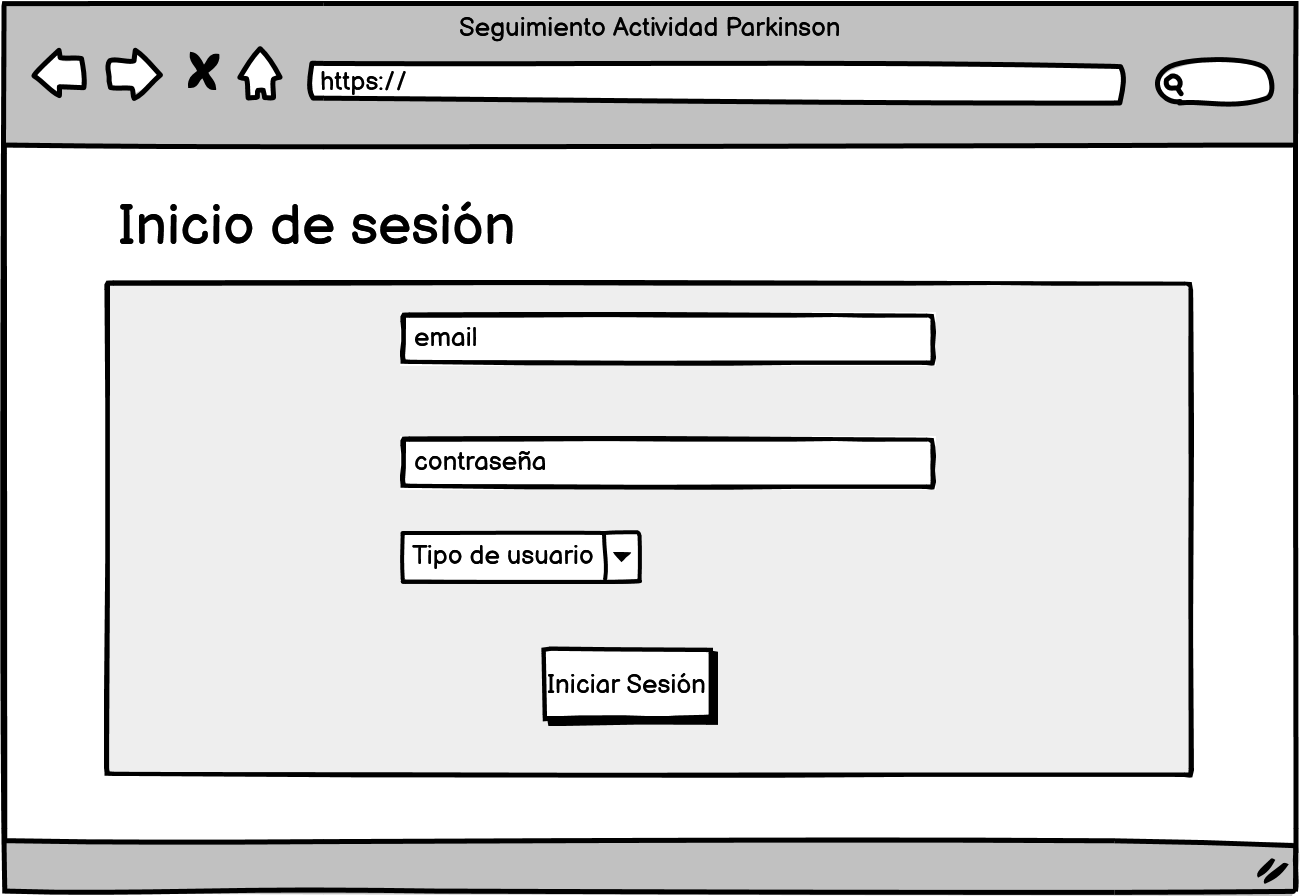
\includegraphics[width=1\textwidth]{img/UI_Wireframes/UI_CU-1_Iniciar sesión.png}
    \caption{Iniciar sesión}
    \label{fig:Iniciar sesión}
\end{figure}

% Confirmar operación
\begin{figure}[h]
    \centering
    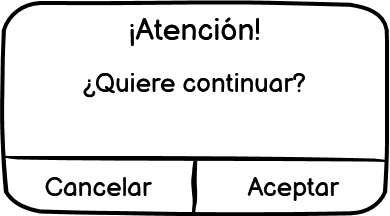
\includegraphics[width=0.4\textwidth]{img/UI_Wireframes/UI_CU-2_Confirmar operación.png}
    \caption{Confirmar operación}
    \label{fig:Confirmar operación}
\end{figure}

% Consulta y gestión de usuarios
\begin{figure}[h]
    \centering
    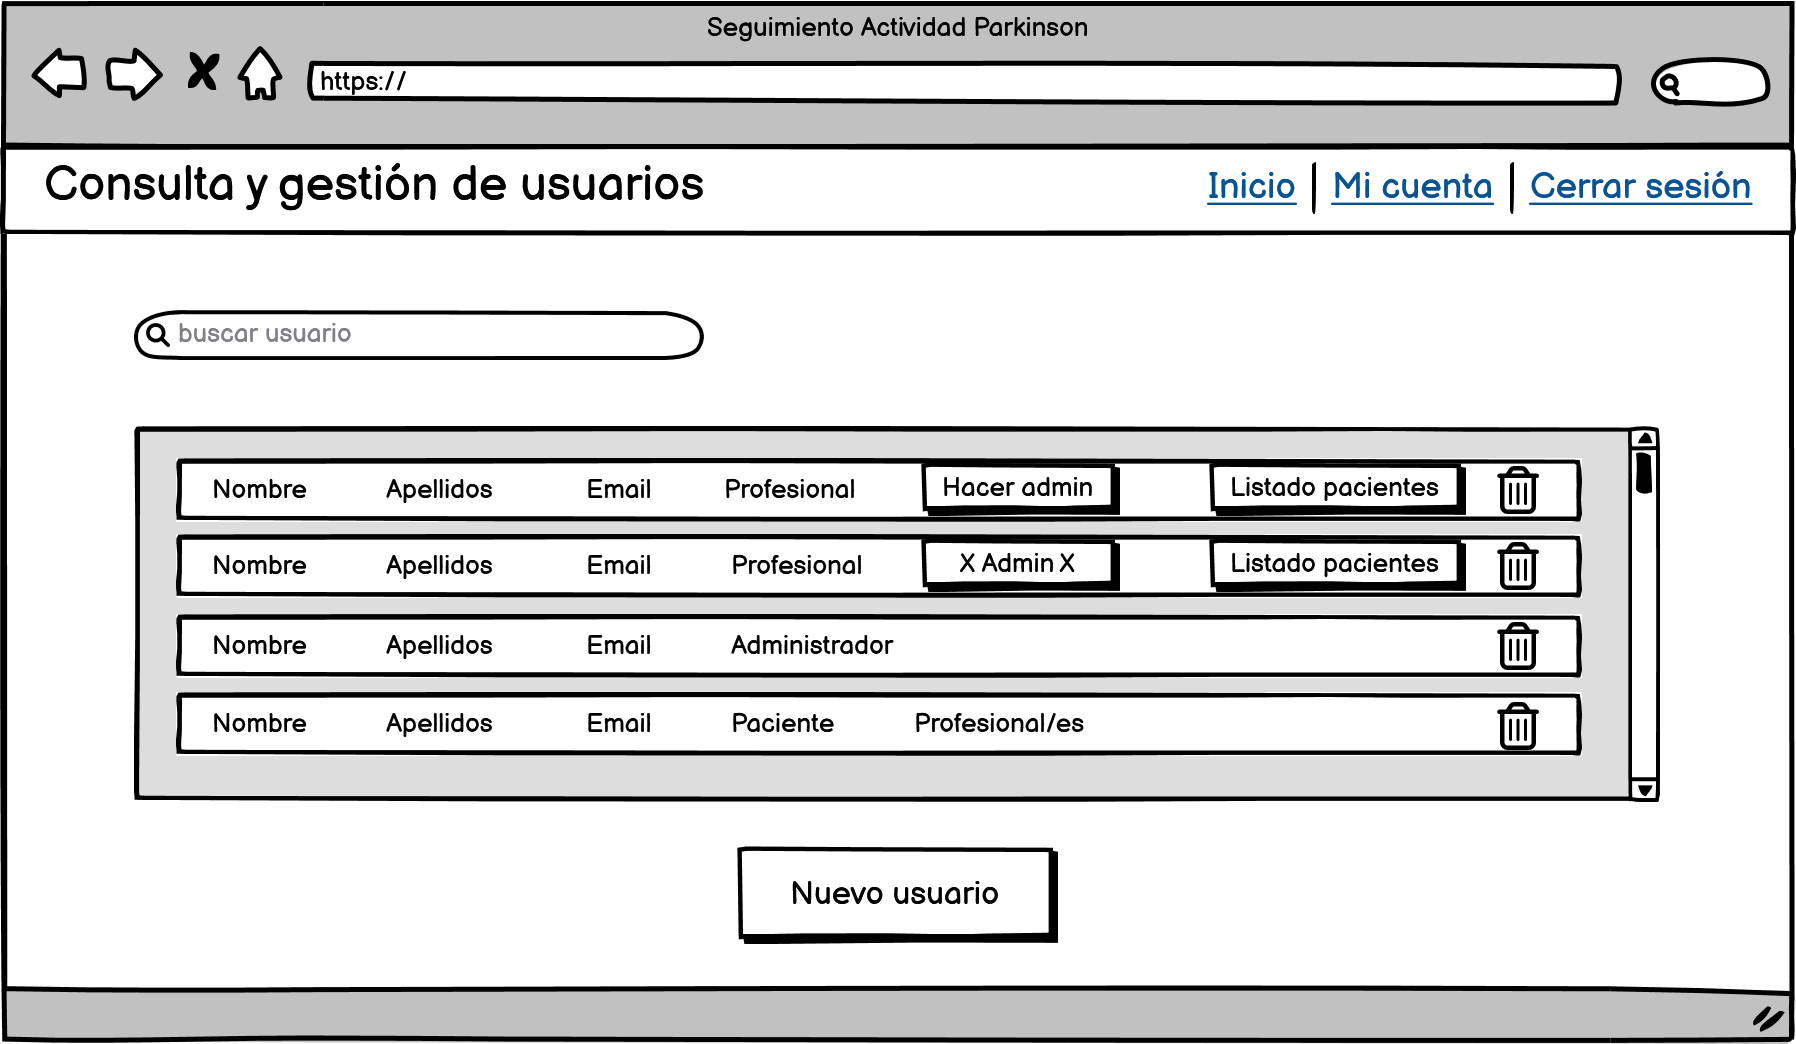
\includegraphics[width=1\textwidth]{img/UI_Wireframes/UI_CU-7_Consulta y gestión de usuarios.png}
    \caption{Consulta y gestión de usuarios}
    \label{fig:Consulta y gestión de usuarios}
\end{figure}

% Crear usuario
\begin{figure}[h]
    \centering
    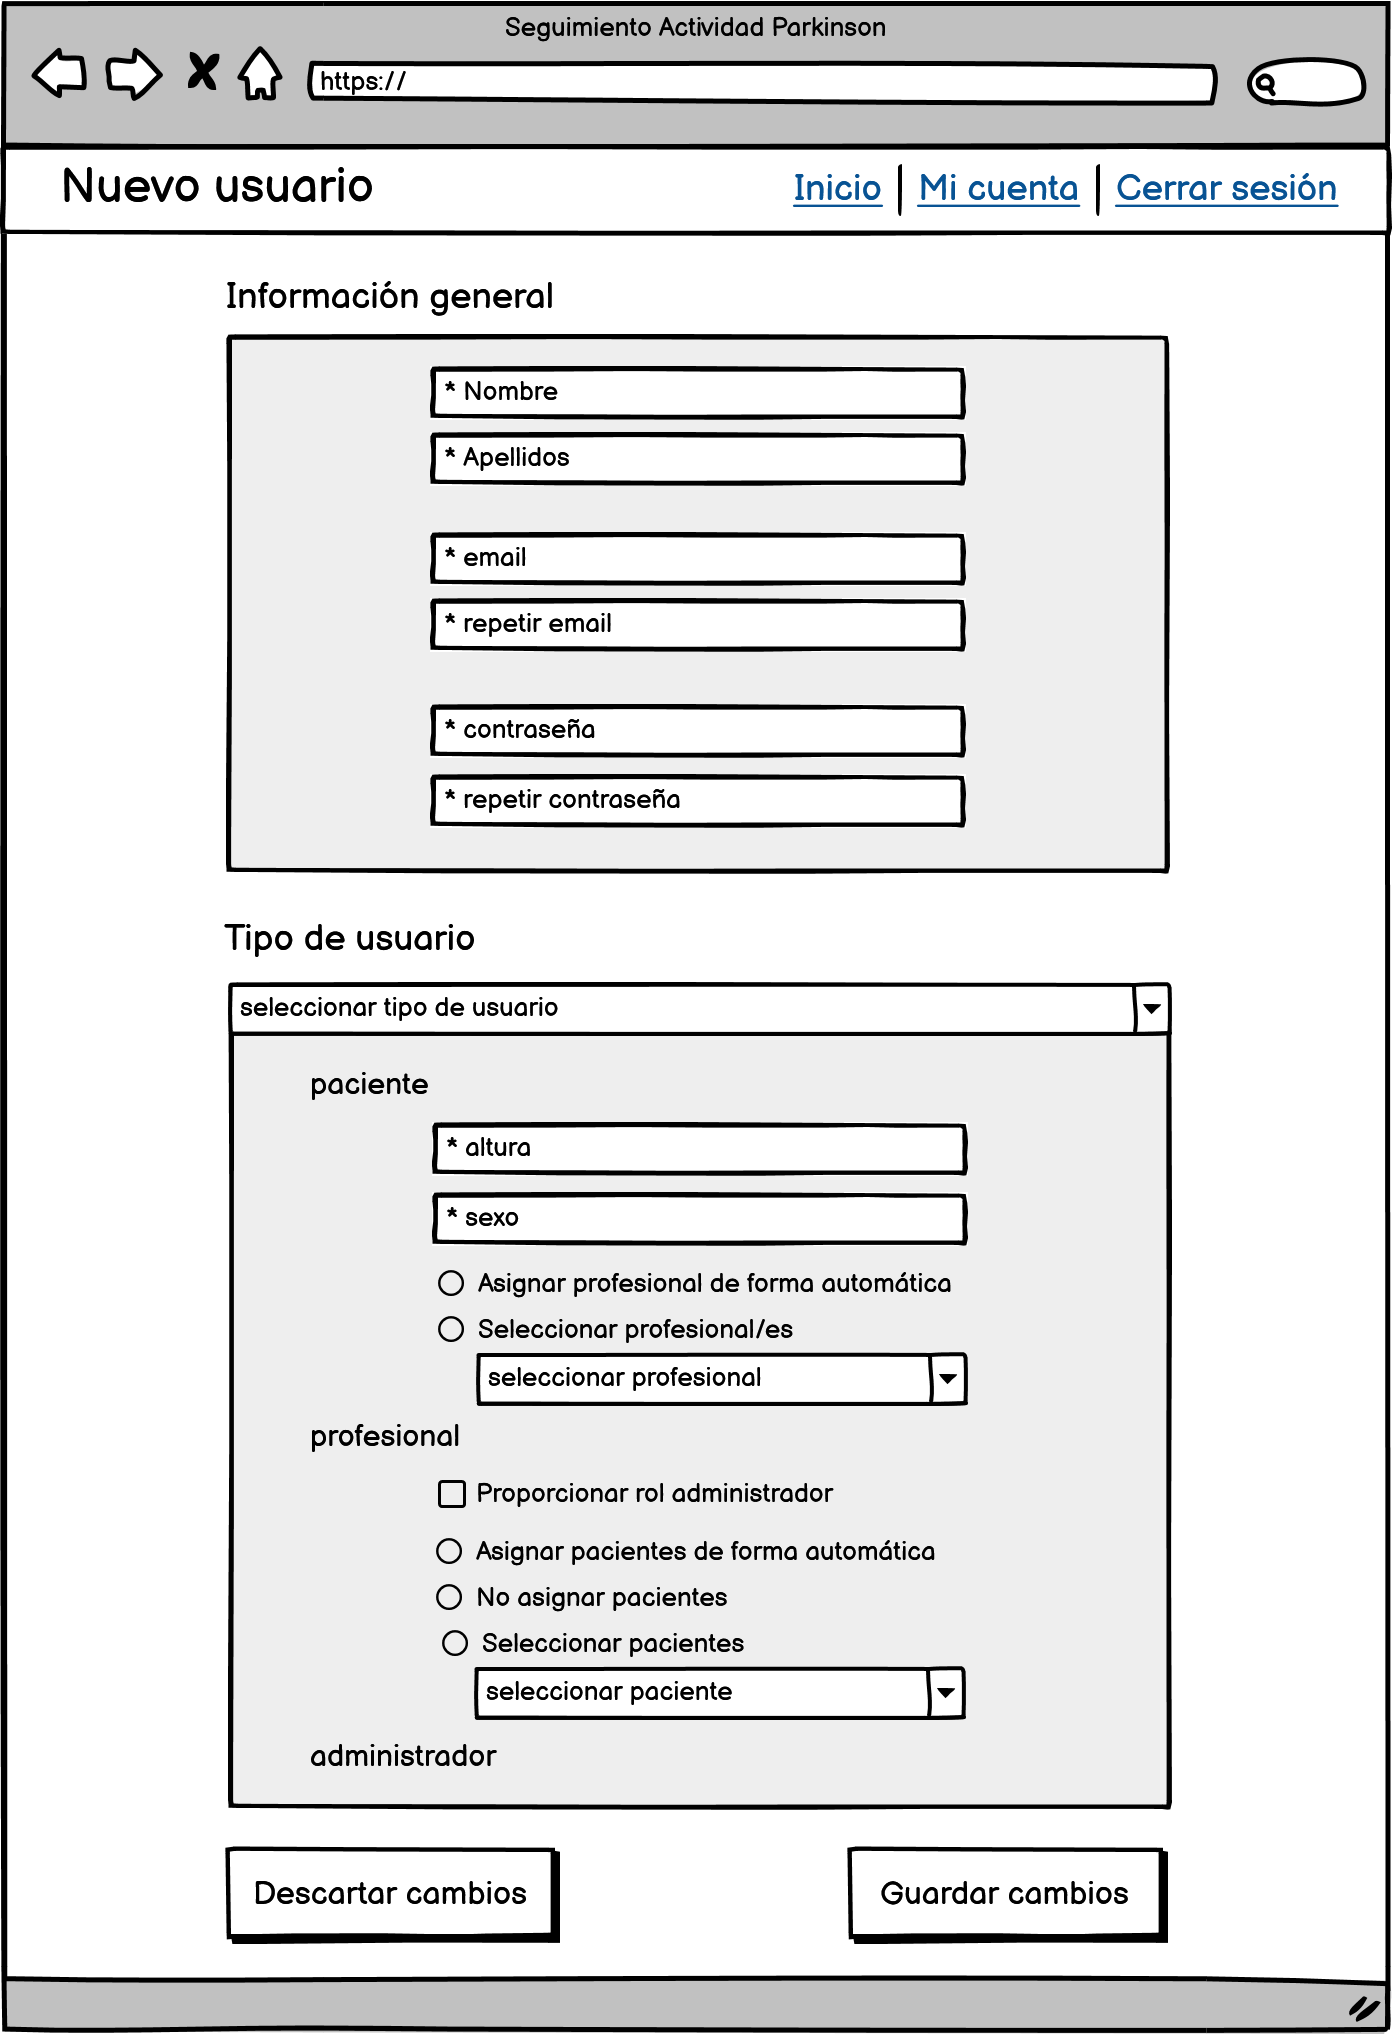
\includegraphics[width=1\textwidth]{img/UI_Wireframes/UI_CU-9_Crear usuario.png}
    \caption{Crear usuario}
    \label{fig:Crear usuario}
\end{figure}

% Consultar lista de pacientes
\begin{figure}[h]
    \centering
    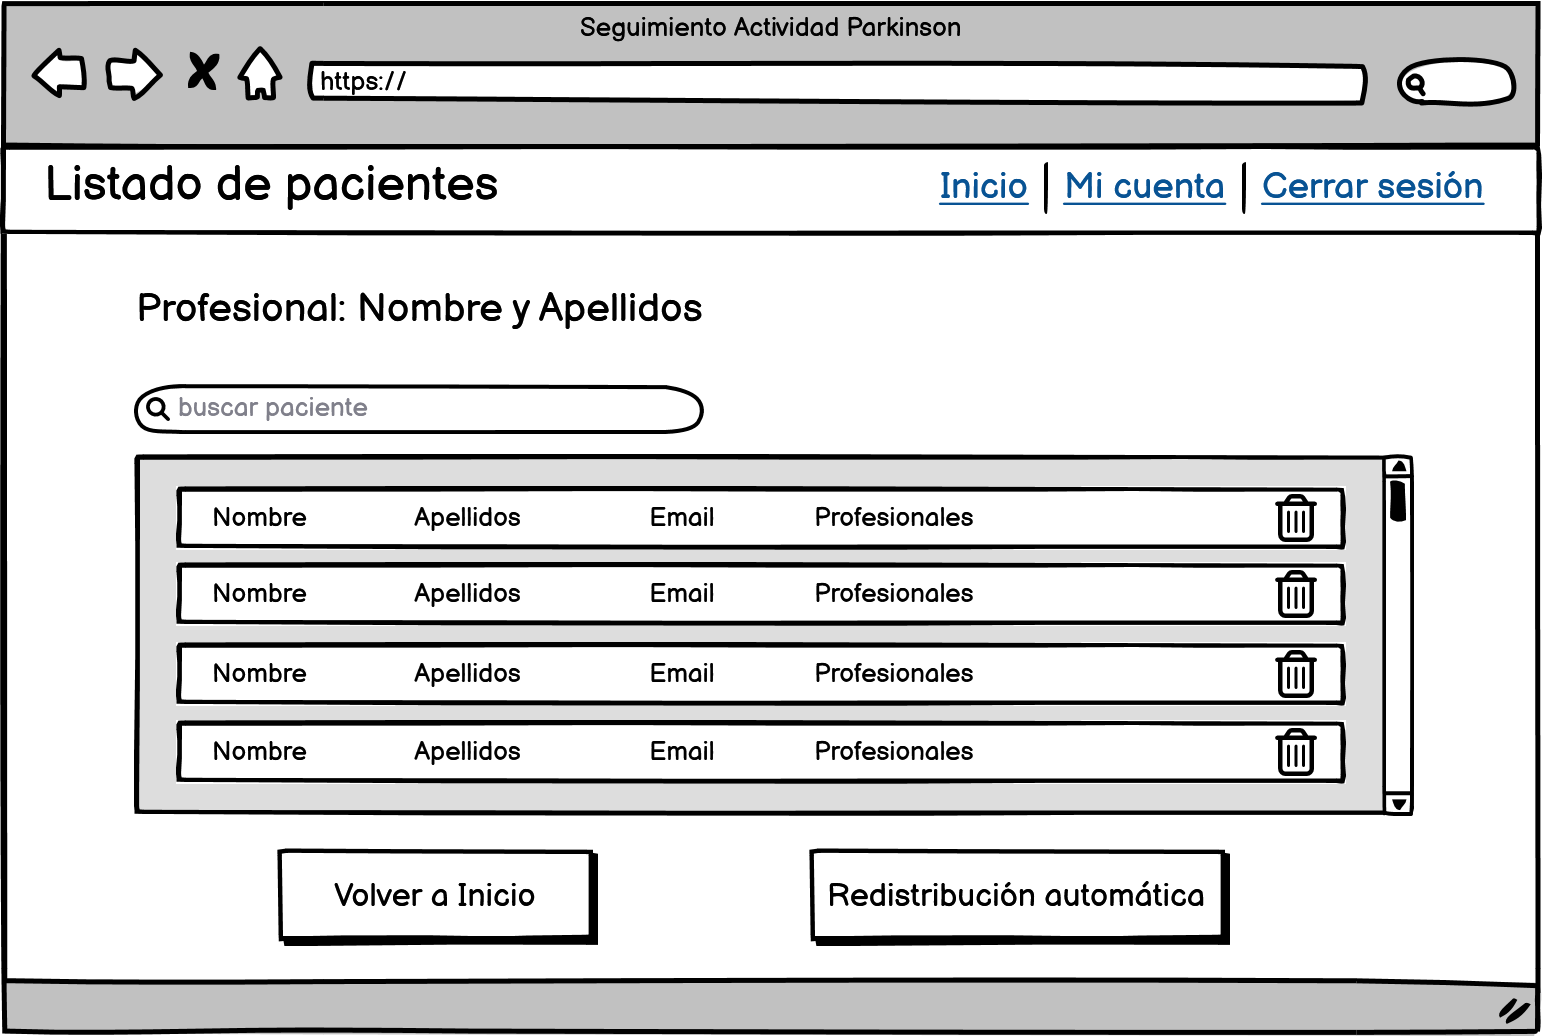
\includegraphics[width=1\textwidth]{img/UI_Wireframes/UI_CU-15_Consultar lista de pacientes.png}
    \caption{Consultar lista de pacientes}
    \label{fig:Consultar lista de pacientes}
\end{figure}

% Consultar información personal y otras operaciones
\begin{figure}[h]
    \centering
    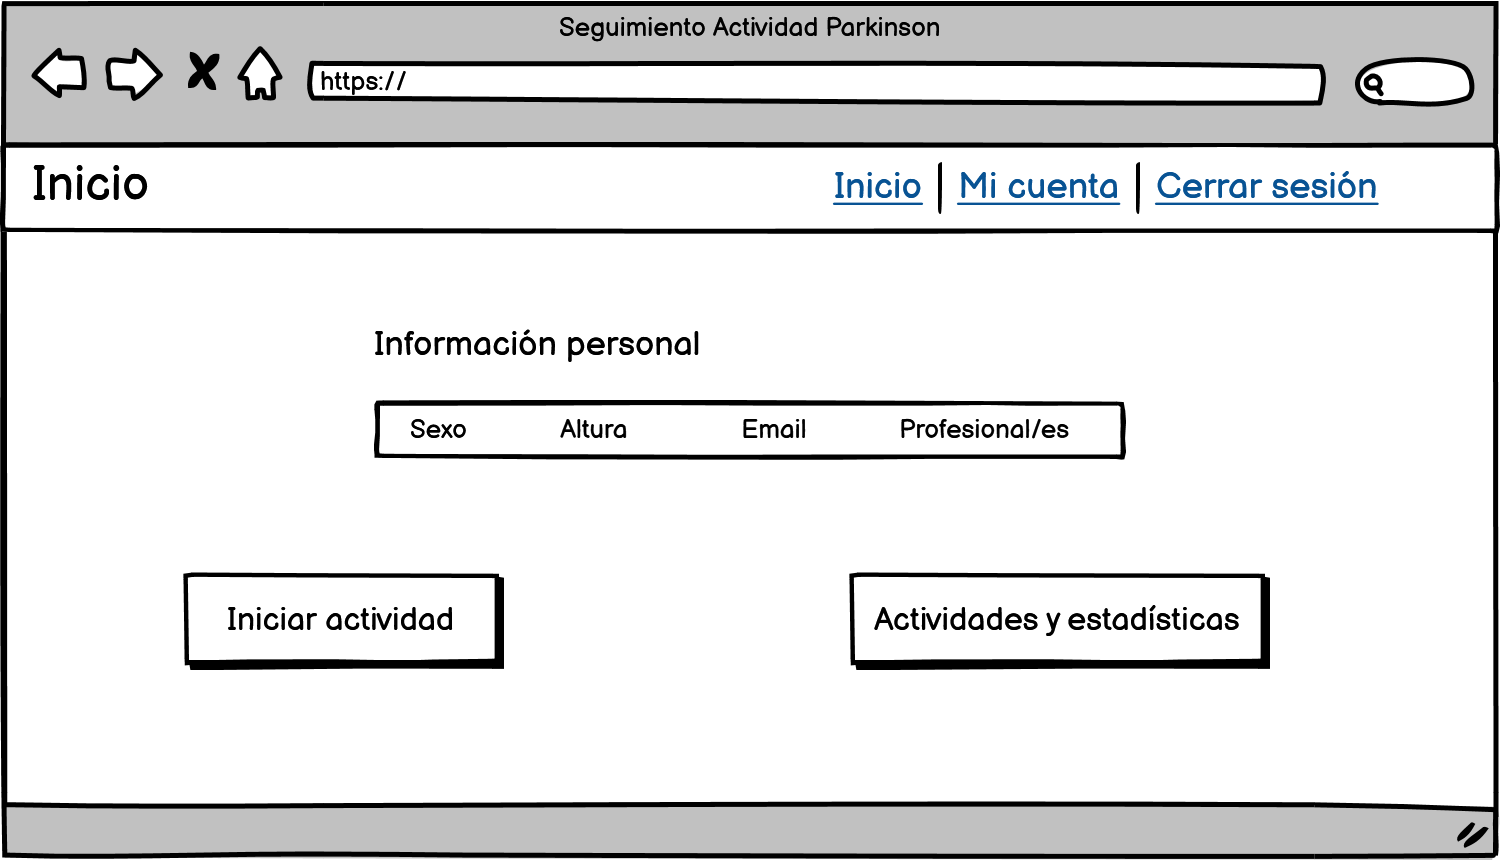
\includegraphics[width=1\textwidth]{img/UI_Wireframes/UI_CU-17_Consultar info personal y otras actividades.png}
    \caption{Consultar información personal y otras actividades}
    \label{fig:Consultar info personal y otras actividades}
\end{figure}

% Iniciar actividad
\begin{figure}[h]
    \centering
    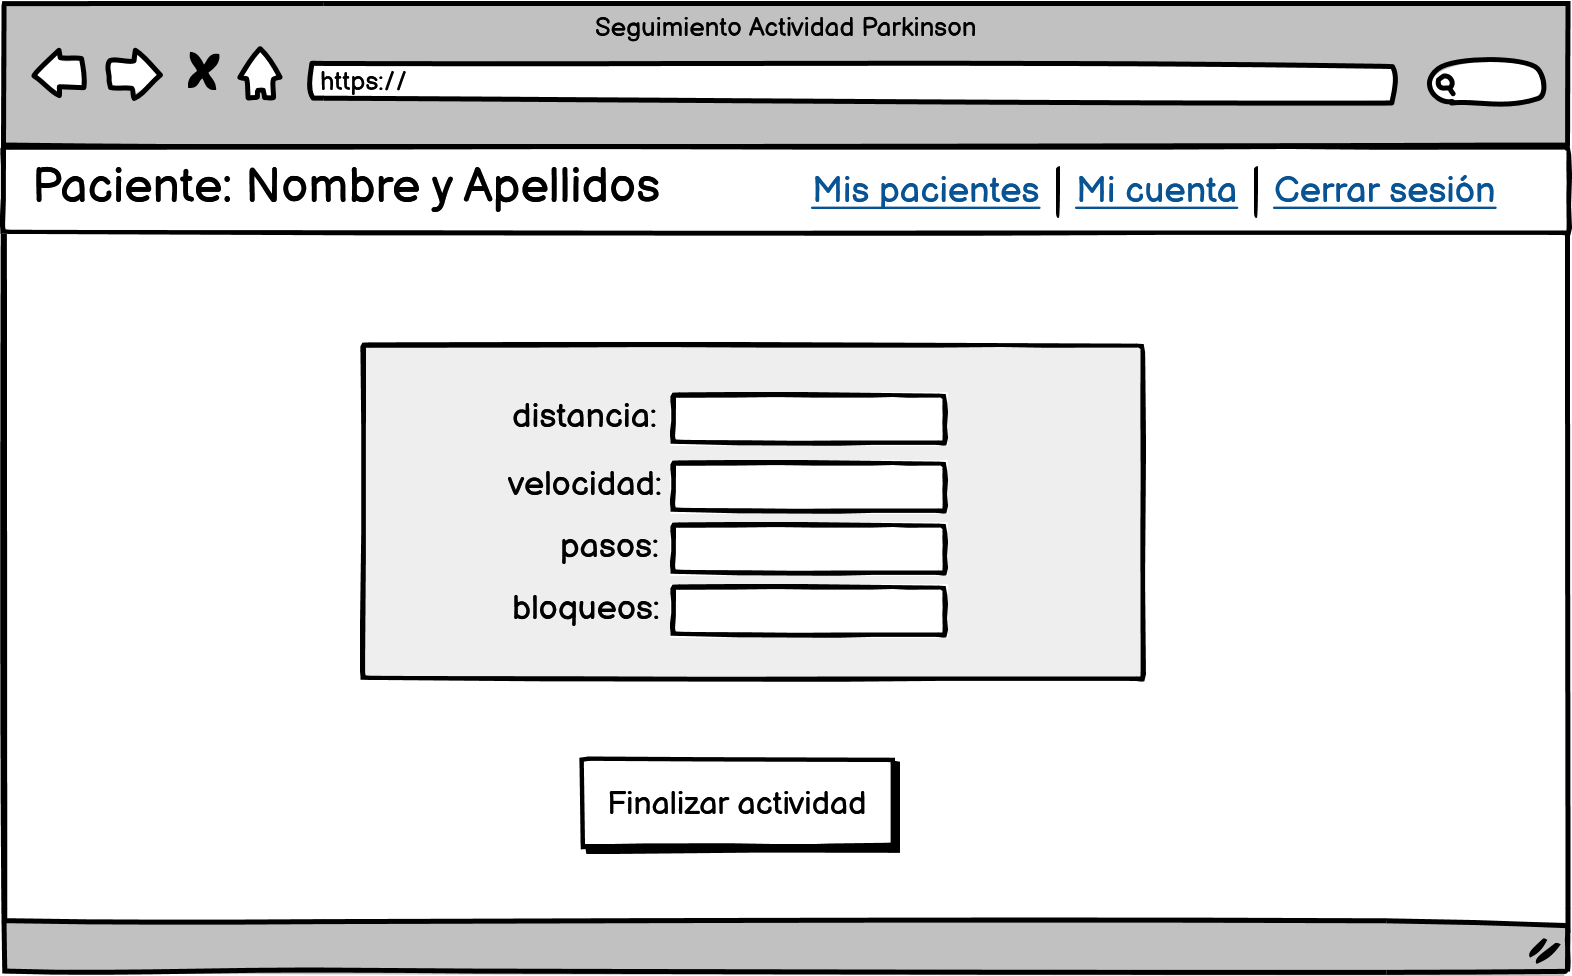
\includegraphics[width=1\textwidth]{img/UI_Wireframes/UI_CU-19_Iniciar actividad.png}
    \caption{Iniciar actividad}
    \label{fig:Iniciar actividad}
\end{figure}

% Consultar actividades y estadísticas (Paciente)
\begin{figure}[h]
    \centering
    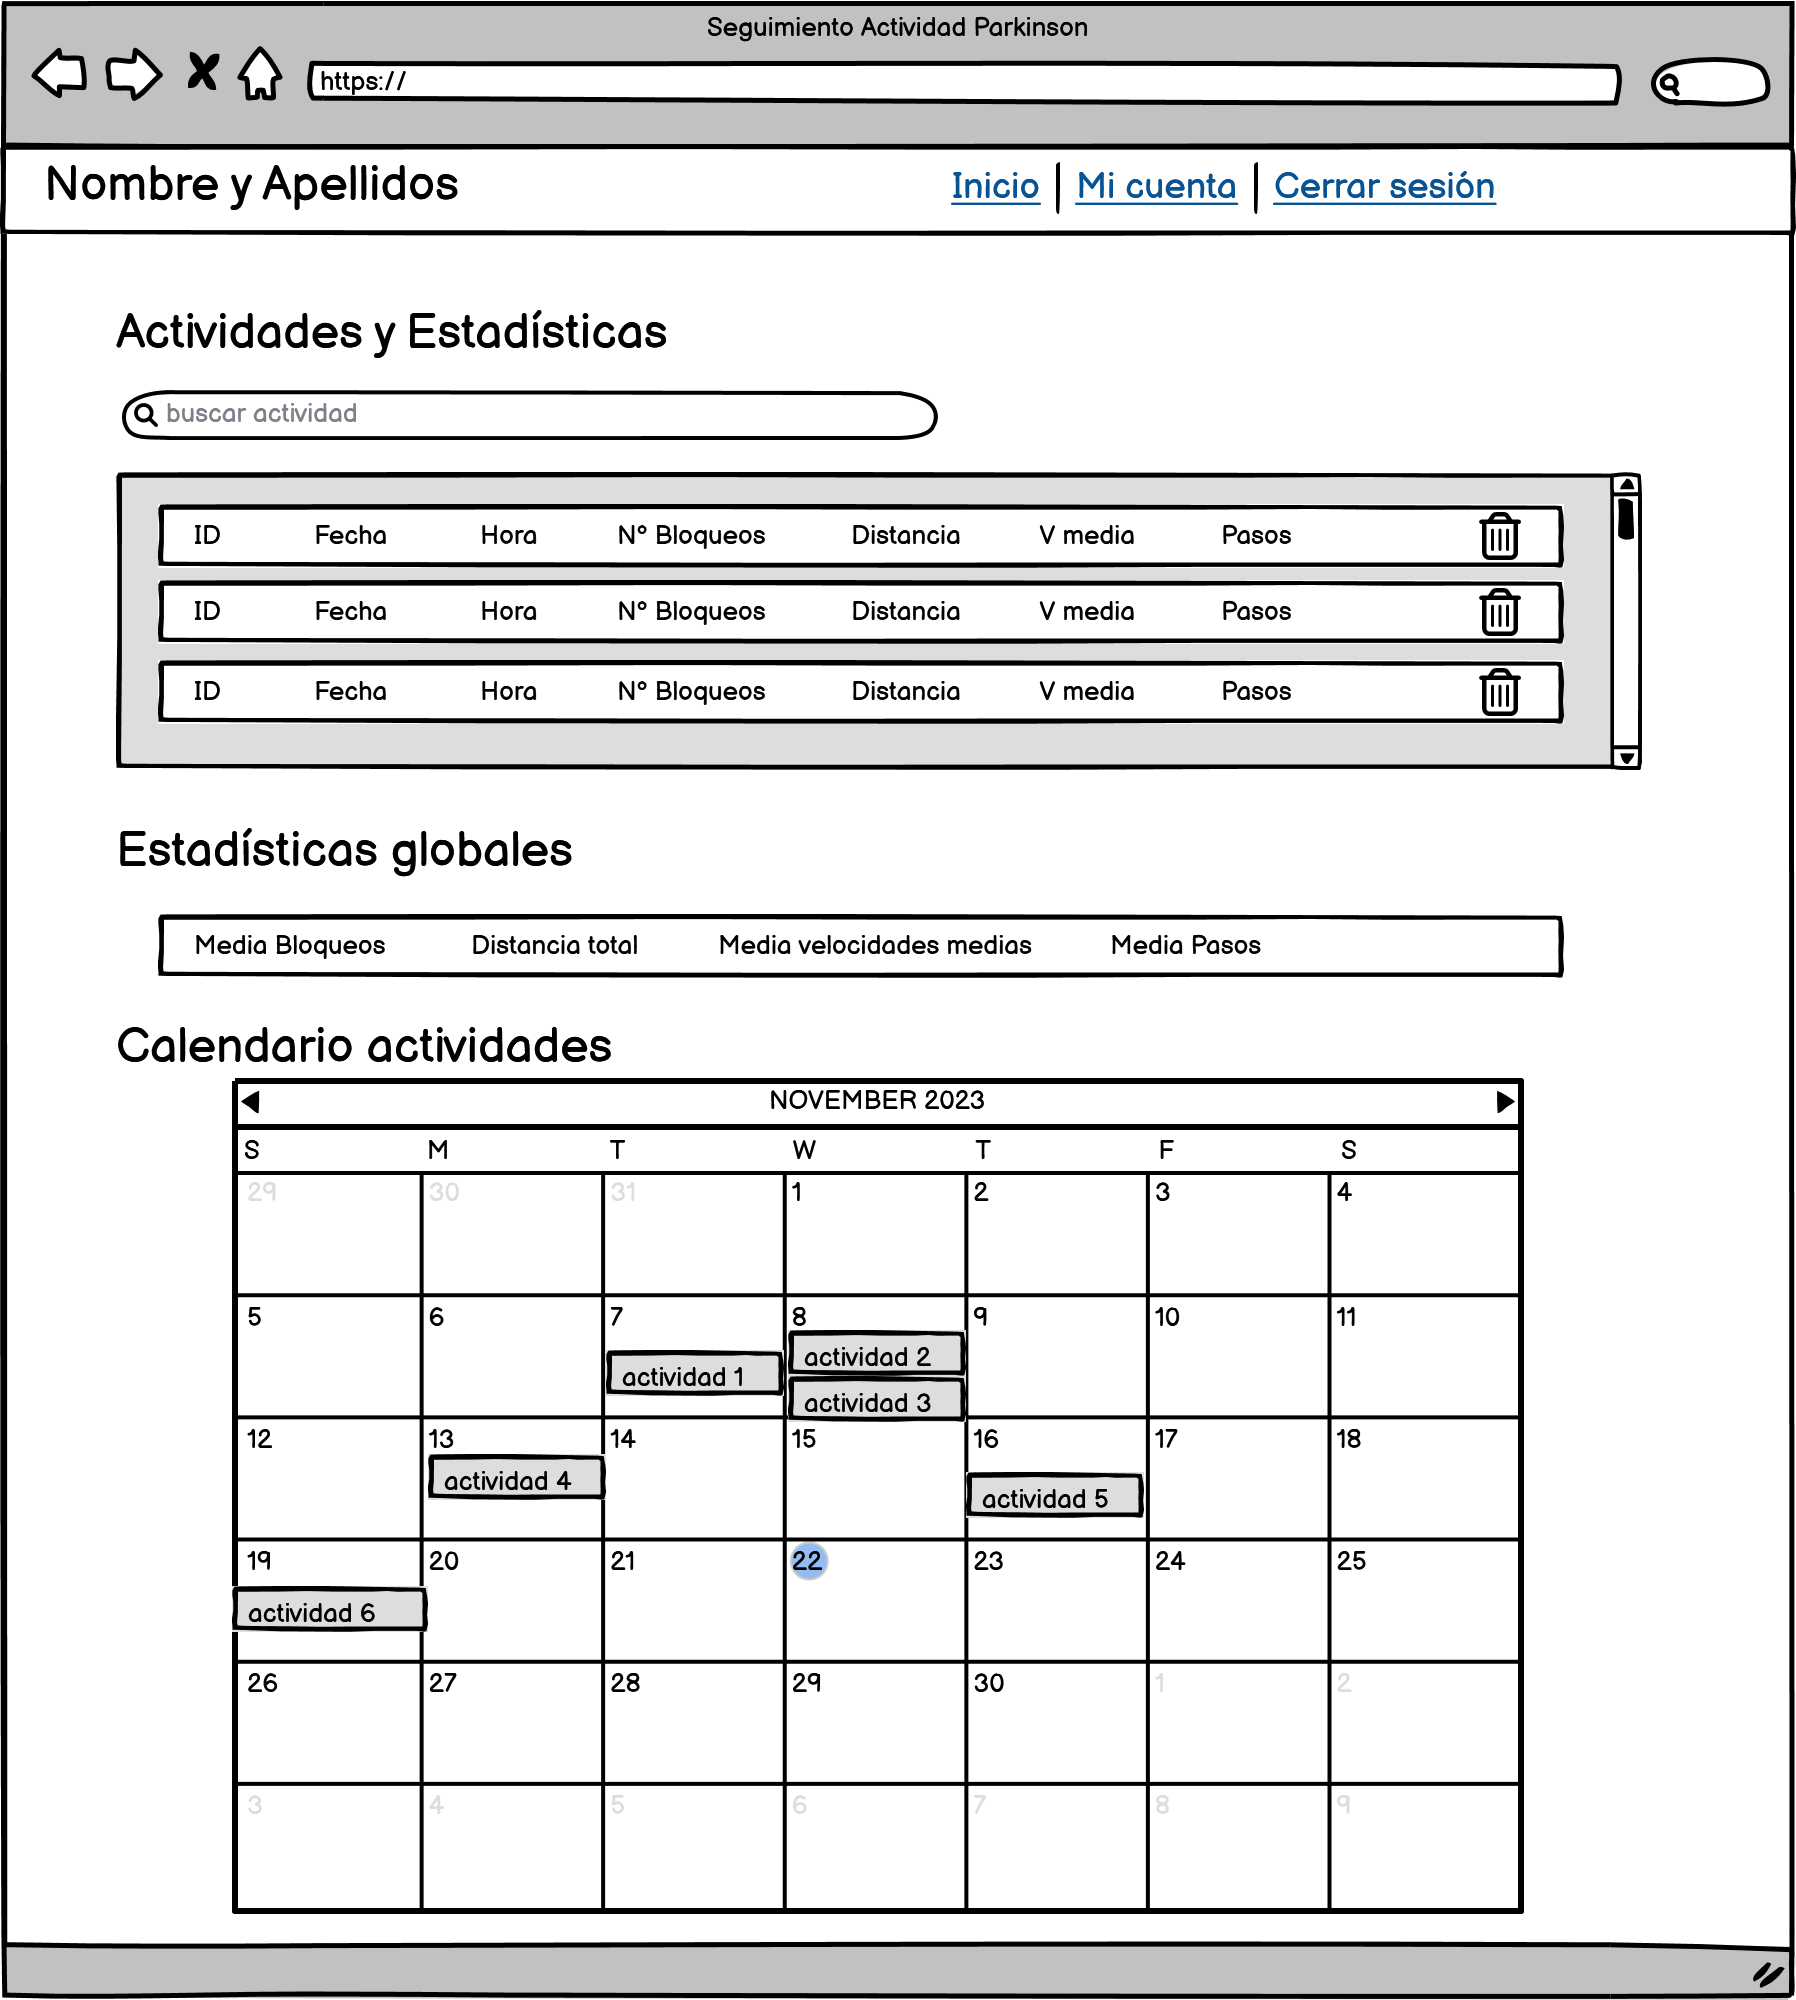
\includegraphics[width=1\textwidth]{img/UI_Wireframes/UI_CU-23_Pac-Consultar actividades y estadísticas (Alternate 323x) (Alternate 323x).png}
    \caption{Consultar actividades y estadísticas (Paciente)}
    \label{fig:Consultar actividades y estadísticas (Paciente)}
\end{figure}

% Consultar actividades y estadísticas (Profesional)
\begin{figure}[h]
    \centering
    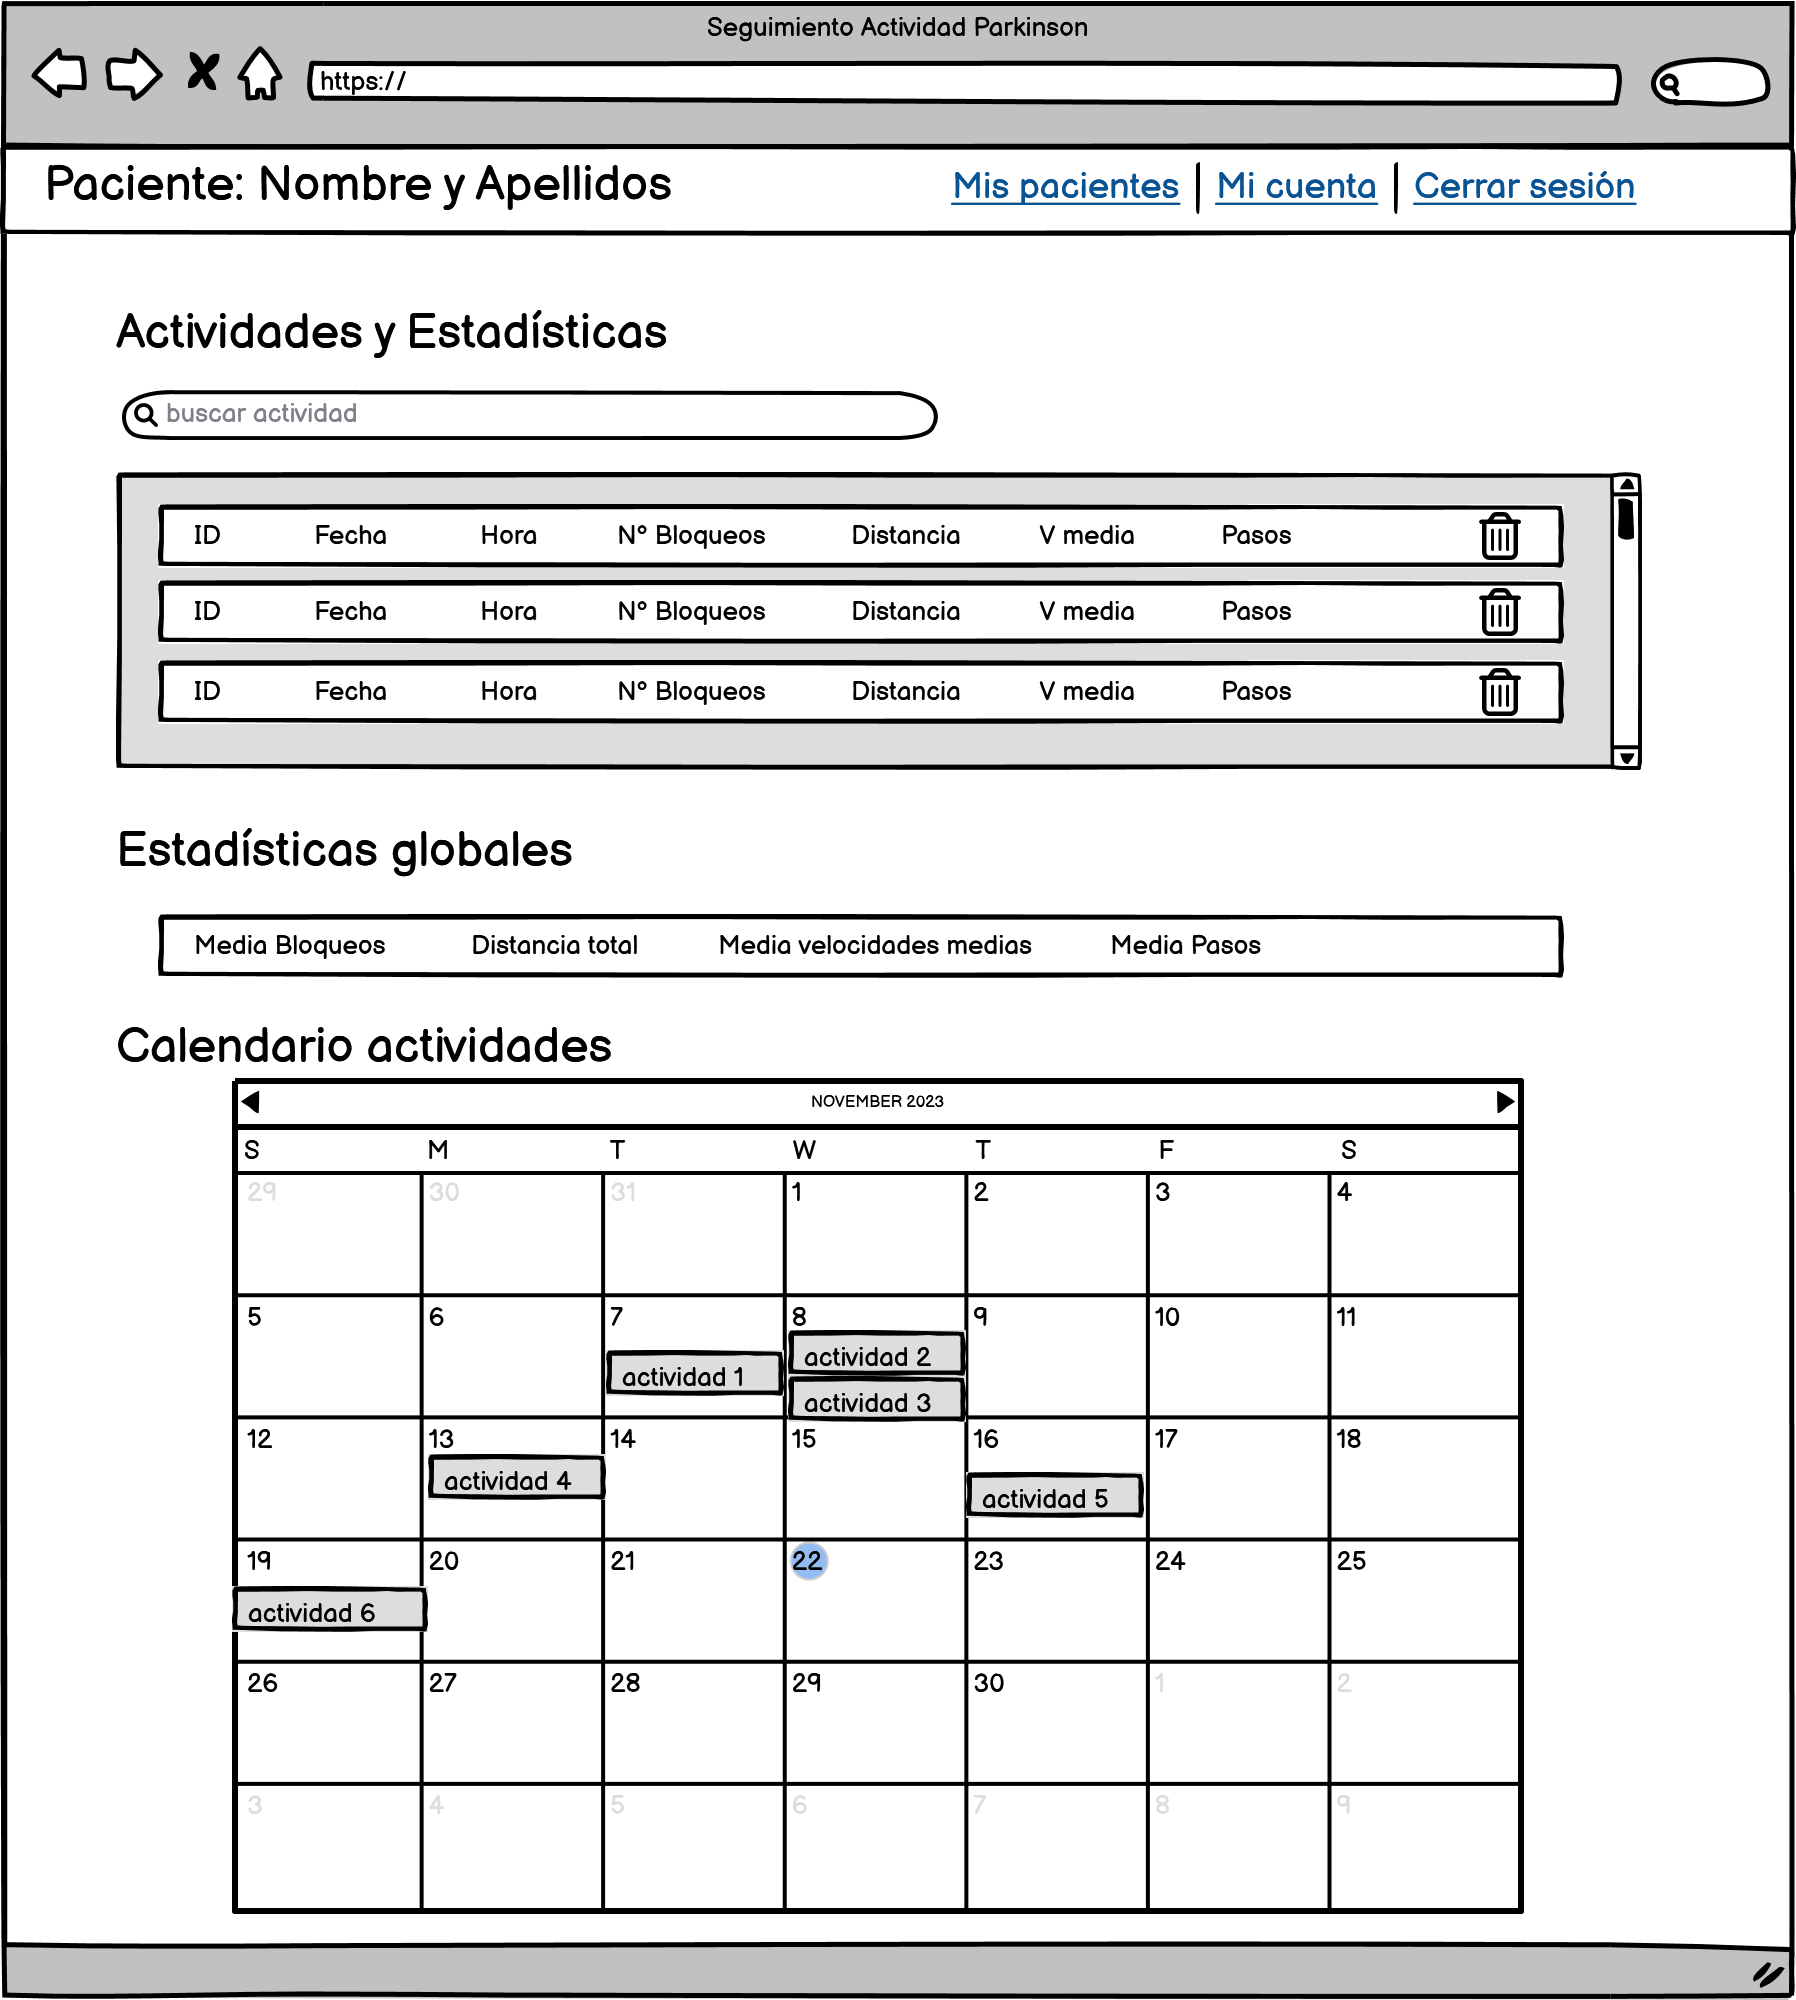
\includegraphics[width=1\textwidth]{img/UI_Wireframes/UI_CU-23_Prof-Consultar actividades y estadísticas.png}
    \caption{Consultar actividades y estadísticas (Profesional)}
    \label{fig:Consultar actividades y estadísticas (Profesional)}
\end{figure}

% Consulta y gestión de pacientes
\begin{figure}[h]
    \centering
    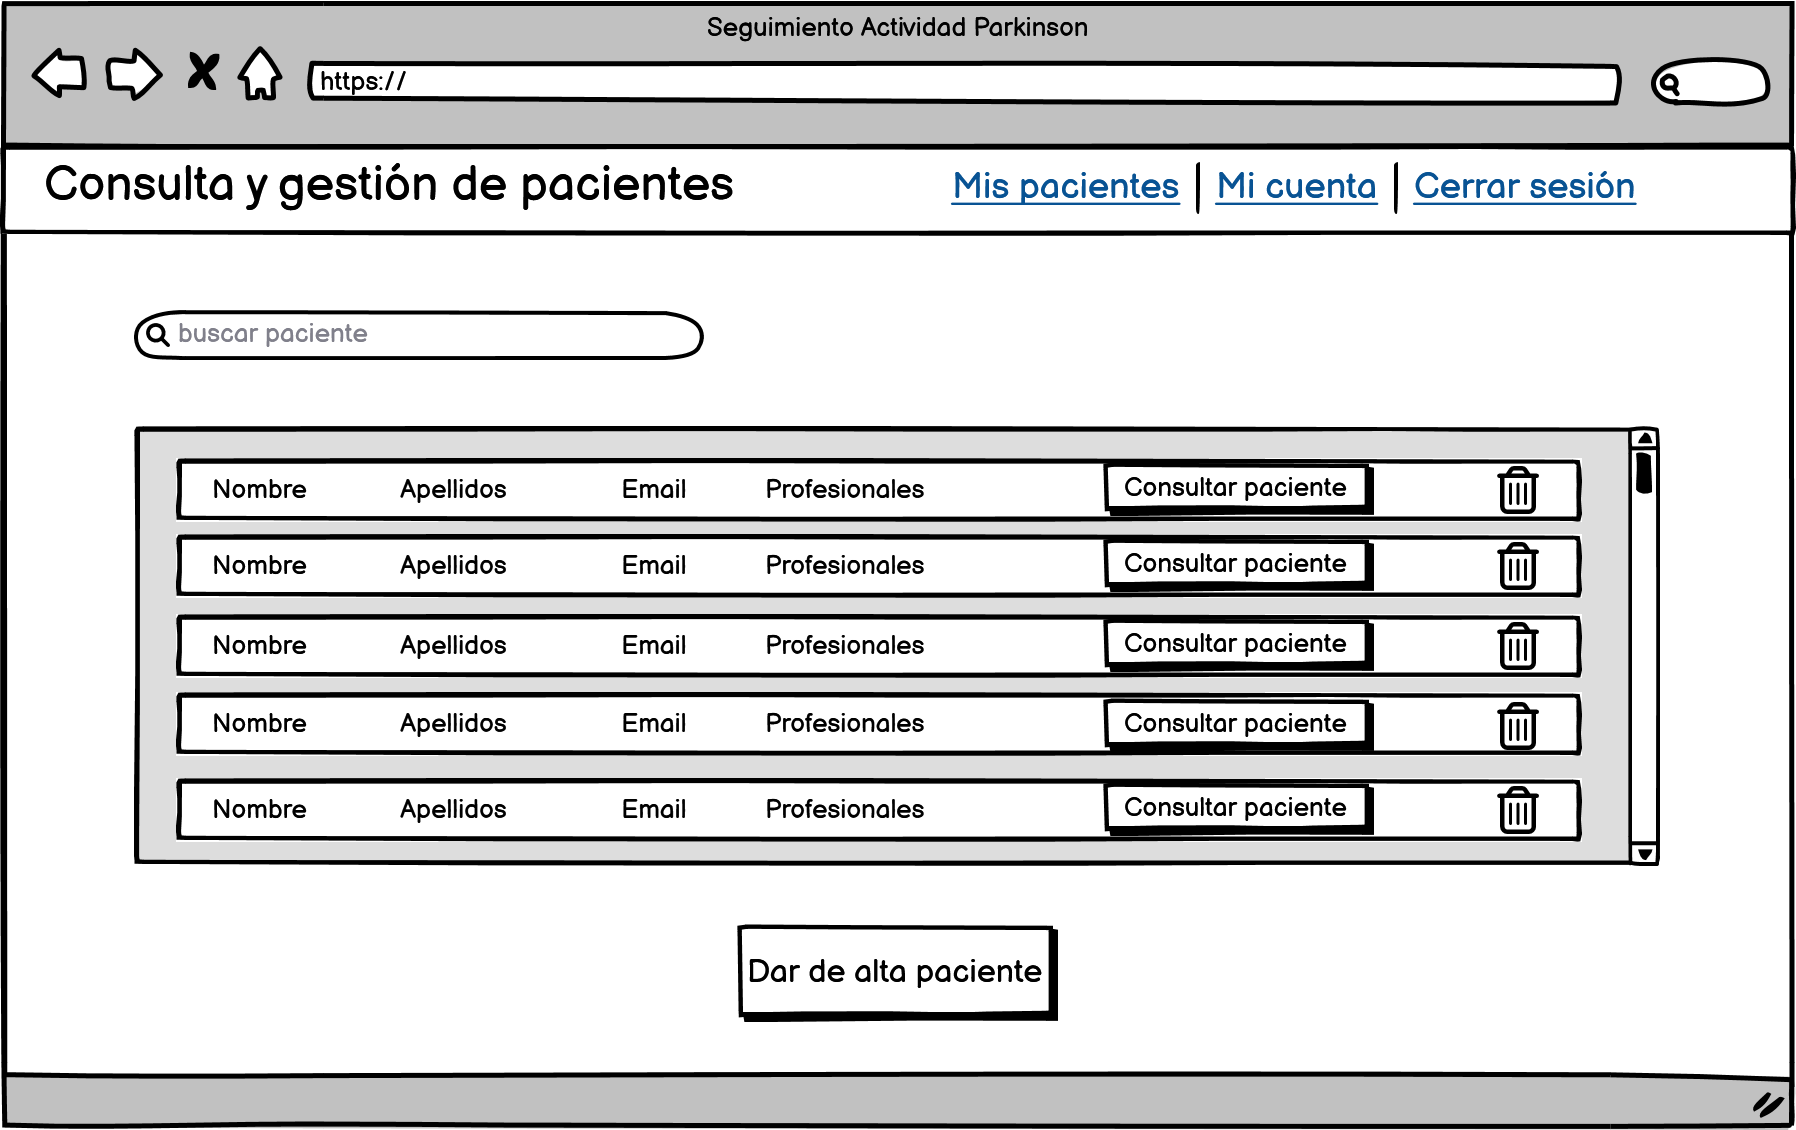
\includegraphics[width=1\textwidth]{img/UI_Wireframes/UI_CU-26_Consulta y gestion de pacientes.png}
    \caption{Consulta y gestión de pacientes}
    \label{fig:Consulta y gestión de pacientes}
\end{figure}

% Crear paciente
\begin{figure}[h]
    \centering
    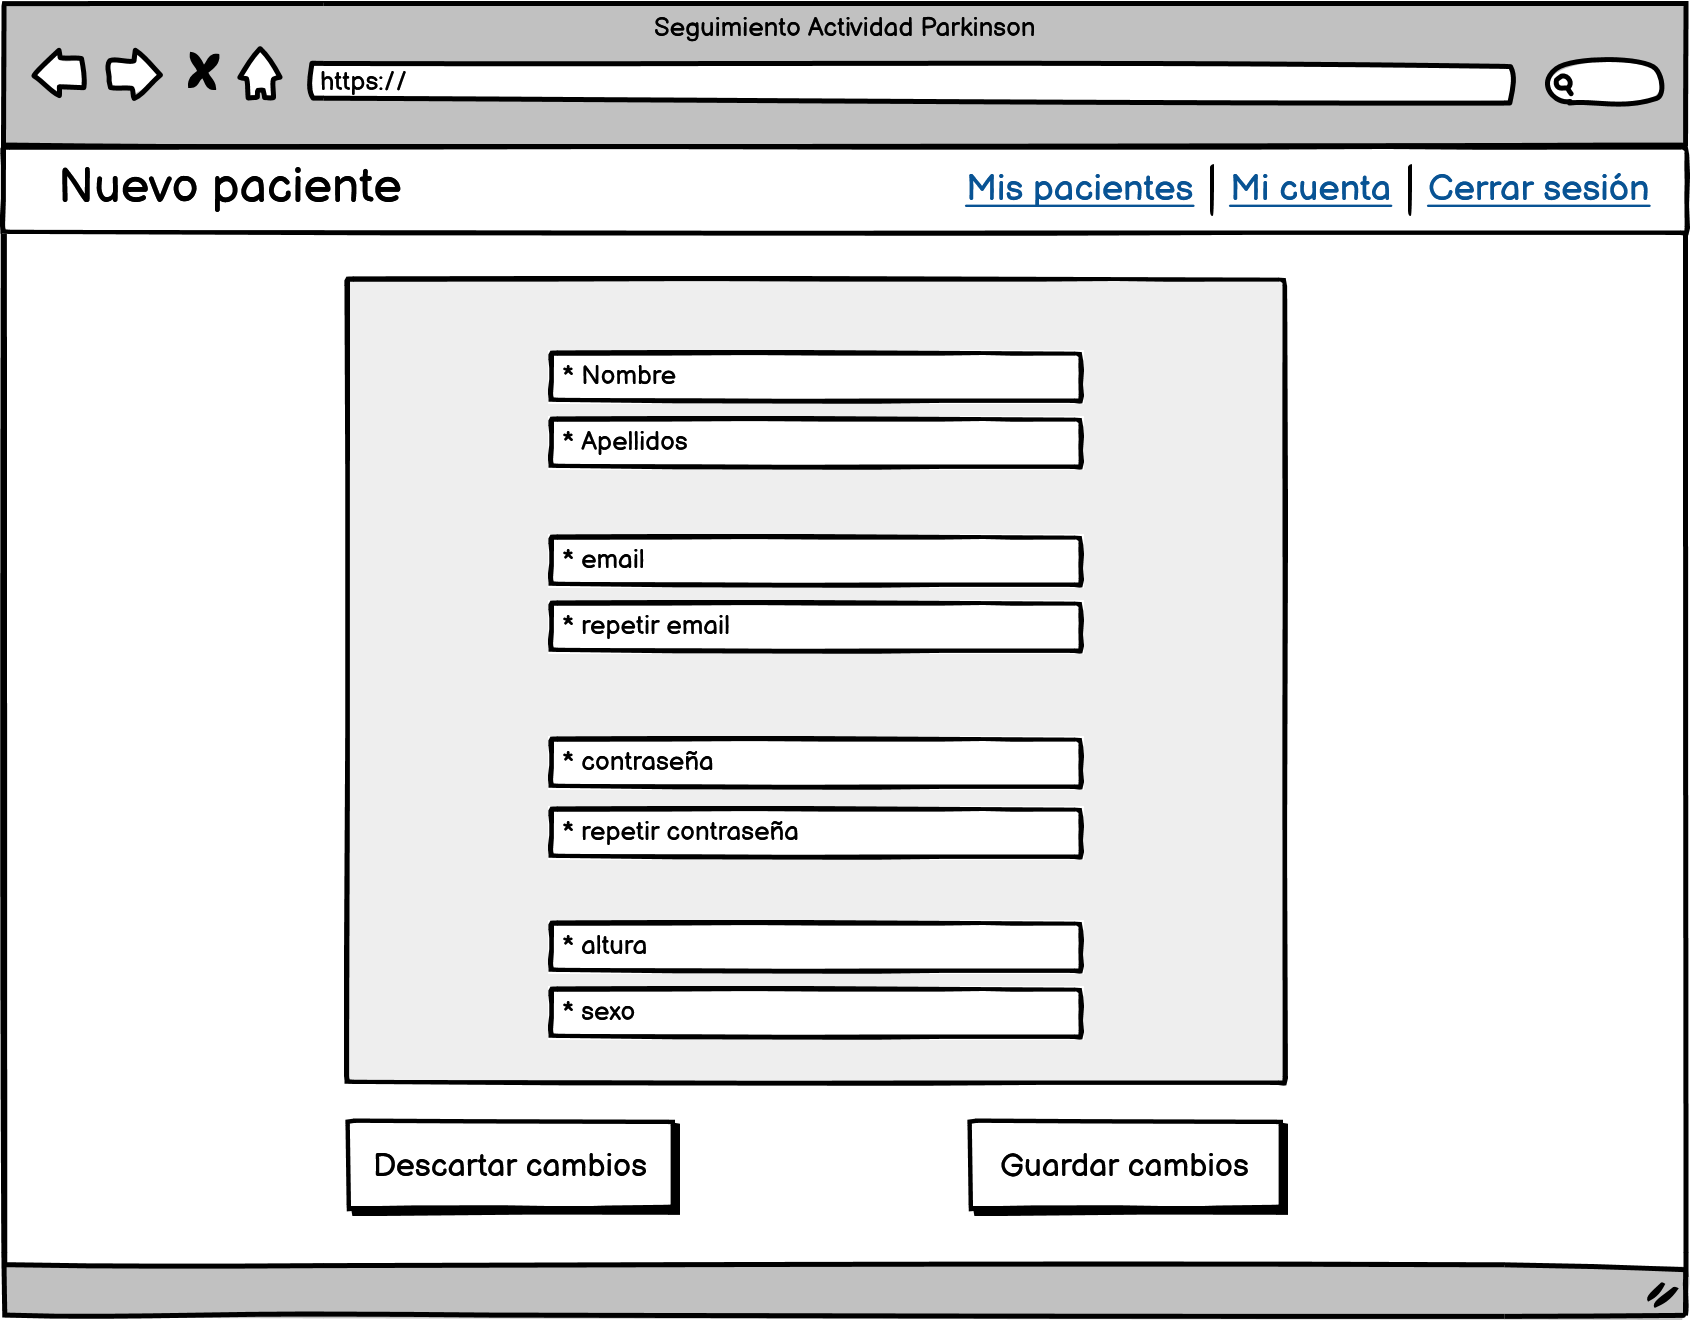
\includegraphics[width=1\textwidth]{img/UI_Wireframes/UI_CU-28_Crear paciente.png}
    \caption{Crear paciente}
    \label{fig:Crear paciente}
\end{figure}

% Visualizar paciente
\begin{figure}[h]
    \centering
    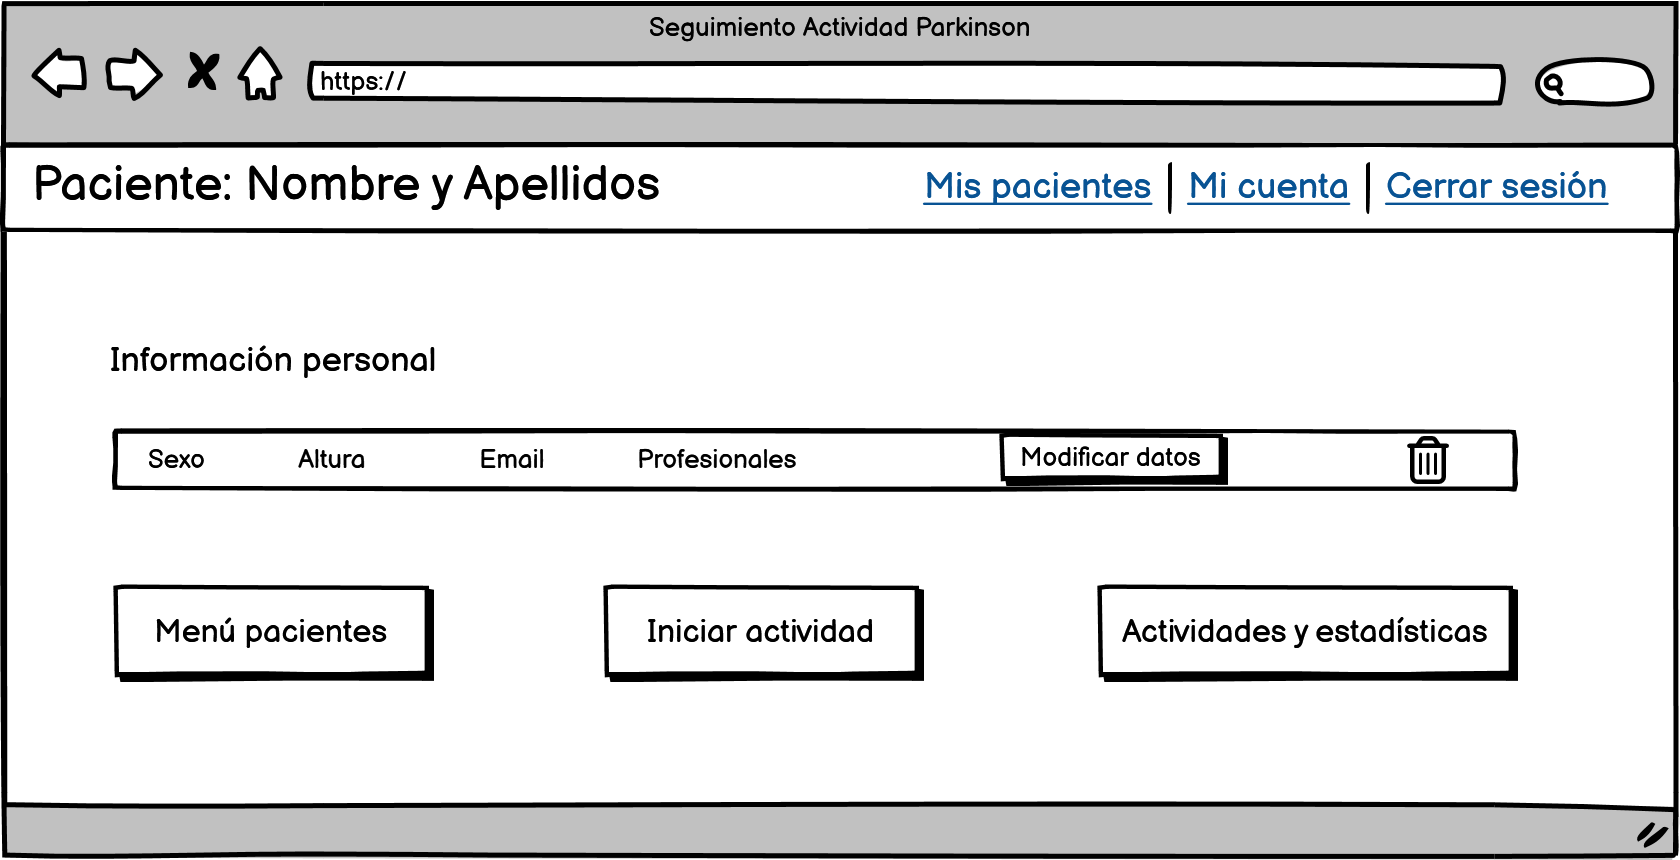
\includegraphics[width=1\textwidth]{img/UI_Wireframes/UI_CU-30_Visualizar paciente.png}
    \caption{Visualizar paciente}
    \label{fig:Visualizar paciente}
\end{figure}